% Options for packages loaded elsewhere
% Options for packages loaded elsewhere
\PassOptionsToPackage{unicode}{hyperref}
\PassOptionsToPackage{hyphens}{url}
%
\documentclass[
  11pt,
  letterpaper,
]{book}
\usepackage{xcolor}
\usepackage{amsmath,amssymb}
\setcounter{secnumdepth}{4}
\usepackage{iftex}
\ifPDFTeX
  \usepackage[T1]{fontenc}
  \usepackage[utf8]{inputenc}
  \usepackage{textcomp} % provide euro and other symbols
\else % if luatex or xetex
  \usepackage{unicode-math} % this also loads fontspec
  \defaultfontfeatures{Scale=MatchLowercase}
  \defaultfontfeatures[\rmfamily]{Ligatures=TeX,Scale=1}
\fi
\usepackage{lmodern}
\ifPDFTeX\else
  % xetex/luatex font selection
\fi
% Use upquote if available, for straight quotes in verbatim environments
\IfFileExists{upquote.sty}{\usepackage{upquote}}{}
\IfFileExists{microtype.sty}{% use microtype if available
  \usepackage[]{microtype}
  \UseMicrotypeSet[protrusion]{basicmath} % disable protrusion for tt fonts
}{}
\makeatletter
\@ifundefined{KOMAClassName}{% if non-KOMA class
  \IfFileExists{parskip.sty}{%
    \usepackage{parskip}
  }{% else
    \setlength{\parindent}{0pt}
    \setlength{\parskip}{6pt plus 2pt minus 1pt}}
}{% if KOMA class
  \KOMAoptions{parskip=half}}
\makeatother
% Make \paragraph and \subparagraph free-standing
\makeatletter
\ifx\paragraph\undefined\else
  \let\oldparagraph\paragraph
  \renewcommand{\paragraph}{
    \@ifstar
      \xxxParagraphStar
      \xxxParagraphNoStar
  }
  \newcommand{\xxxParagraphStar}[1]{\oldparagraph*{#1}\mbox{}}
  \newcommand{\xxxParagraphNoStar}[1]{\oldparagraph{#1}\mbox{}}
\fi
\ifx\subparagraph\undefined\else
  \let\oldsubparagraph\subparagraph
  \renewcommand{\subparagraph}{
    \@ifstar
      \xxxSubParagraphStar
      \xxxSubParagraphNoStar
  }
  \newcommand{\xxxSubParagraphStar}[1]{\oldsubparagraph*{#1}\mbox{}}
  \newcommand{\xxxSubParagraphNoStar}[1]{\oldsubparagraph{#1}\mbox{}}
\fi
\makeatother

\usepackage{color}
\usepackage{fancyvrb}
\newcommand{\VerbBar}{|}
\newcommand{\VERB}{\Verb[commandchars=\\\{\}]}
\DefineVerbatimEnvironment{Highlighting}{Verbatim}{commandchars=\\\{\}}
% Add ',fontsize=\small' for more characters per line
\usepackage{framed}
\definecolor{shadecolor}{RGB}{241,243,245}
\newenvironment{Shaded}{\begin{snugshade}}{\end{snugshade}}
\newcommand{\AlertTok}[1]{\textcolor[rgb]{0.68,0.00,0.00}{#1}}
\newcommand{\AnnotationTok}[1]{\textcolor[rgb]{0.37,0.37,0.37}{#1}}
\newcommand{\AttributeTok}[1]{\textcolor[rgb]{0.40,0.45,0.13}{#1}}
\newcommand{\BaseNTok}[1]{\textcolor[rgb]{0.68,0.00,0.00}{#1}}
\newcommand{\BuiltInTok}[1]{\textcolor[rgb]{0.00,0.23,0.31}{#1}}
\newcommand{\CharTok}[1]{\textcolor[rgb]{0.13,0.47,0.30}{#1}}
\newcommand{\CommentTok}[1]{\textcolor[rgb]{0.37,0.37,0.37}{#1}}
\newcommand{\CommentVarTok}[1]{\textcolor[rgb]{0.37,0.37,0.37}{\textit{#1}}}
\newcommand{\ConstantTok}[1]{\textcolor[rgb]{0.56,0.35,0.01}{#1}}
\newcommand{\ControlFlowTok}[1]{\textcolor[rgb]{0.00,0.23,0.31}{\textbf{#1}}}
\newcommand{\DataTypeTok}[1]{\textcolor[rgb]{0.68,0.00,0.00}{#1}}
\newcommand{\DecValTok}[1]{\textcolor[rgb]{0.68,0.00,0.00}{#1}}
\newcommand{\DocumentationTok}[1]{\textcolor[rgb]{0.37,0.37,0.37}{\textit{#1}}}
\newcommand{\ErrorTok}[1]{\textcolor[rgb]{0.68,0.00,0.00}{#1}}
\newcommand{\ExtensionTok}[1]{\textcolor[rgb]{0.00,0.23,0.31}{#1}}
\newcommand{\FloatTok}[1]{\textcolor[rgb]{0.68,0.00,0.00}{#1}}
\newcommand{\FunctionTok}[1]{\textcolor[rgb]{0.28,0.35,0.67}{#1}}
\newcommand{\ImportTok}[1]{\textcolor[rgb]{0.00,0.46,0.62}{#1}}
\newcommand{\InformationTok}[1]{\textcolor[rgb]{0.37,0.37,0.37}{#1}}
\newcommand{\KeywordTok}[1]{\textcolor[rgb]{0.00,0.23,0.31}{\textbf{#1}}}
\newcommand{\NormalTok}[1]{\textcolor[rgb]{0.00,0.23,0.31}{#1}}
\newcommand{\OperatorTok}[1]{\textcolor[rgb]{0.37,0.37,0.37}{#1}}
\newcommand{\OtherTok}[1]{\textcolor[rgb]{0.00,0.23,0.31}{#1}}
\newcommand{\PreprocessorTok}[1]{\textcolor[rgb]{0.68,0.00,0.00}{#1}}
\newcommand{\RegionMarkerTok}[1]{\textcolor[rgb]{0.00,0.23,0.31}{#1}}
\newcommand{\SpecialCharTok}[1]{\textcolor[rgb]{0.37,0.37,0.37}{#1}}
\newcommand{\SpecialStringTok}[1]{\textcolor[rgb]{0.13,0.47,0.30}{#1}}
\newcommand{\StringTok}[1]{\textcolor[rgb]{0.13,0.47,0.30}{#1}}
\newcommand{\VariableTok}[1]{\textcolor[rgb]{0.07,0.07,0.07}{#1}}
\newcommand{\VerbatimStringTok}[1]{\textcolor[rgb]{0.13,0.47,0.30}{#1}}
\newcommand{\WarningTok}[1]{\textcolor[rgb]{0.37,0.37,0.37}{\textit{#1}}}

\usepackage{longtable,booktabs,array}
\newcounter{none} % for unnumbered tables
\usepackage{calc} % for calculating minipage widths
% Correct order of tables after \paragraph or \subparagraph
\usepackage{etoolbox}
\makeatletter
\patchcmd\longtable{\par}{\if@noskipsec\mbox{}\fi\par}{}{}
\makeatother
% Allow footnotes in longtable head/foot
\IfFileExists{footnotehyper.sty}{\usepackage{footnotehyper}}{\usepackage{footnote}}
\makesavenoteenv{longtable}
\usepackage{graphicx}
\makeatletter
\newsavebox\pandoc@box
\newcommand*\pandocbounded[1]{% scales image to fit in text height/width
  \sbox\pandoc@box{#1}%
  \Gscale@div\@tempa{\textheight}{\dimexpr\ht\pandoc@box+\dp\pandoc@box\relax}%
  \Gscale@div\@tempb{\linewidth}{\wd\pandoc@box}%
  \ifdim\@tempb\p@<\@tempa\p@\let\@tempa\@tempb\fi% select the smaller of both
  \ifdim\@tempa\p@<\p@\scalebox{\@tempa}{\usebox\pandoc@box}%
  \else\usebox{\pandoc@box}%
  \fi%
}
% Set default figure placement to htbp
\def\fps@figure{htbp}
\makeatother

\ifLuaTeX
  \usepackage{luacolor}
  \usepackage[soul]{lua-ul}
\else
  \usepackage{soul}
\fi

% definitions for citeproc citations
\NewDocumentCommand\citeproctext{}{}
\NewDocumentCommand\citeproc{mm}{%
  \begingroup\def\citeproctext{#2}\cite{#1}\endgroup}
\makeatletter
 % allow citations to break across lines
 \let\@cite@ofmt\@firstofone
 % avoid brackets around text for \cite:
 \def\@biblabel#1{}
 \def\@cite#1#2{{#1\if@tempswa , #2\fi}}
\makeatother
\newlength{\cslhangindent}
\setlength{\cslhangindent}{1.5em}
\newlength{\csllabelwidth}
\setlength{\csllabelwidth}{3em}
\newenvironment{CSLReferences}[2] % #1 hanging-indent, #2 entry-spacing
 {\begin{list}{}{%
  \setlength{\itemindent}{0pt}
  \setlength{\leftmargin}{0pt}
  \setlength{\parsep}{0pt}
  % turn on hanging indent if param 1 is 1
  \ifodd #1
   \setlength{\leftmargin}{\cslhangindent}
   \setlength{\itemindent}{-1\cslhangindent}
  \fi
  % set entry spacing
  \setlength{\itemsep}{#2\baselineskip}}}
 {\end{list}}
\usepackage{calc}
\newcommand{\CSLBlock}[1]{\hfill\break\parbox[t]{\linewidth}{\strut\ignorespaces#1\strut}}
\newcommand{\CSLLeftMargin}[1]{\parbox[t]{\csllabelwidth}{\strut#1\strut}}
\newcommand{\CSLRightInline}[1]{\parbox[t]{\linewidth - \csllabelwidth}{\strut#1\strut}}
\newcommand{\CSLIndent}[1]{\hspace{\cslhangindent}#1}



\setlength{\emergencystretch}{3em} % prevent overfull lines

\providecommand{\tightlist}{%
  \setlength{\itemsep}{0pt}\setlength{\parskip}{0pt}}



 


\makeatletter
\@ifpackageloaded{bookmark}{}{\usepackage{bookmark}}
\makeatother
\makeatletter
\@ifpackageloaded{caption}{}{\usepackage{caption}}
\AtBeginDocument{%
\ifdefined\contentsname
  \renewcommand*\contentsname{Table of contents}
\else
  \newcommand\contentsname{Table of contents}
\fi
\ifdefined\listfigurename
  \renewcommand*\listfigurename{List of Figures}
\else
  \newcommand\listfigurename{List of Figures}
\fi
\ifdefined\listtablename
  \renewcommand*\listtablename{List of Tables}
\else
  \newcommand\listtablename{List of Tables}
\fi
\ifdefined\figurename
  \renewcommand*\figurename{Figure}
\else
  \newcommand\figurename{Figure}
\fi
\ifdefined\tablename
  \renewcommand*\tablename{Table}
\else
  \newcommand\tablename{Table}
\fi
}
\@ifpackageloaded{float}{}{\usepackage{float}}
\floatstyle{ruled}
\@ifundefined{c@chapter}{\newfloat{codelisting}{h}{lop}}{\newfloat{codelisting}{h}{lop}[chapter]}
\floatname{codelisting}{Listing}
\newcommand*\listoflistings{\listof{codelisting}{List of Listings}}
\makeatother
\makeatletter
\makeatother
\makeatletter
\@ifpackageloaded{caption}{}{\usepackage{caption}}
\@ifpackageloaded{subcaption}{}{\usepackage{subcaption}}
\makeatother
\usepackage{bookmark}
\IfFileExists{xurl.sty}{\usepackage{xurl}}{} % add URL line breaks if available
\urlstyle{same}
\hypersetup{
  pdftitle={Build-It-Yourself: Low-Cost Systems for Field Ecophysiology},
  pdfauthor={Mathias Hoffmann; Milan Shay Kretzschmar; Reena Macagga; Wael Al Hamwi; Adrian Dahlmann; Maren Dubbert; David Dubbert; John Marshall; Michael Asante; Geoffrey Sossa},
  hidelinks,
  pdfcreator={LaTeX via pandoc}}


\title{Build-It-Yourself: Low-Cost Systems for Field Ecophysiology}
\usepackage{etoolbox}
\makeatletter
\providecommand{\subtitle}[1]{% add subtitle to \maketitle
  \apptocmd{\@title}{\par {\large #1 \par}}{}{}
}
\makeatother
\subtitle{An Open Handbook for DIY Environmental Measurement Systems}
\author{Mathias Hoffmann \and Milan Shay Kretzschmar \and Reena
Macagga \and Wael Al Hamwi \and Adrian Dahlmann \and Maren
Dubbert \and David Dubbert \and John Marshall \and Michael
Asante \and Geoffrey Sossa}
\date{2026-04-22}
\begin{document}
\frontmatter
\maketitle

\renewcommand*\contentsname{Table of contents}
{
\setcounter{tocdepth}{2}
\tableofcontents
}

\mainmatter
\bookmarksetup{startatroot}

\chapter{Preface}\label{sec-preface}

This handbook is part of the MonksHillLab initiative (integral part of
the
\href{https://www.zalf.de/en/struktur/pb1/ibg/Pages/default.aspx}{Working
Group Ecophysiology of Water and Matter Cycling} of the
\href{https://www.zalf.de/en/Pages/ZALF.aspx}{Leibniz Centre for
Agricultural Landscape Research}) which aims to democratize science by
enabling low-cost, DIY sensor development for environmental monitoring.
It provides step-by-step guidance on building and calibrating sensor
systems using open hardware and widely available components.

The project supports ecophysiological research and the discovery of
sustainable agricultural management practices, particularly in
under-resourced regions and the Global South. By focusing on
reproducibility, accessibility, and practical application, it seeks to
close the gap between research/development and field
implementation/adoption.

This is a living document: users are encouraged to build upon the
existing designs, share adaptations, and contribute new chapters, see
the Section~\ref{sec-contributing} section for more details. Future
versions will include additional low-cost DIY systems and their
integration with the MonksHillLab Logger App. Thus, together, we aim to
grow with that handbook a practical, evolving resource for scientists,
students, and practitioners.

We are currently exploring the idea of organizing a low-cost sensor
summer school and/or online workshop to provide hands-on training,
exchange ideas, and build a global community around DIY environmental
monitoring. If you are interested in participating or helping shape the
format, feel free to get in touch or respond to the
\href{https://docs.google.com/forms/d/e/1FAIpQLSd-lZMnjAK-ll1-eMoKwWdKpjrdHeFioPDRd5Fp-lMQW38EWg/viewform?usp=header}{feedback
link}

\section{Structure of the handbook}\label{sec-structure}

This handbook provides open-source, low-cost designs for field-based
ecophysiological measurement systems in agricultural research. It is
intended to support researchers, practitioners, and students in building
and deploying affordable monitoring tools that can be adapted to a wide
range of field conditions. To provide structure and clarity, the
handbook is organized around three key domains of ecophysiological
monitoring: (1) environmental variables (e.g., air temperature,
humidity, radiation, soil moisture), (2) plant health and development
(e.g., leaf temperature, chlorophyll status, canopy reflectance), and
(3) biogeochemical cycles (e.g., evapotranspiration (ET), CO₂ and CH₄
fluxes, nutrient dynamics). These categories reflect increasing system
complexity---from relatively simple measurements of ambient conditions
to more integrated assessments of ecosystem processes. Each chapter
follows the same practical structure---covering use cases, required
materials, wiring diagrams, step-by-step assembly, calibration, and
code---making it easy to adapt and implement these systems regardless of
technical background.

\section{Contributing}\label{sec-contributing}

You're very welcome to share your improvements/chapters. Just email the
author (mathias.hoffmann@zalf.de) and submit an update.

\section{Whats New?}\label{sec-whats-new}

\textbf{Version 2.1} introduces the EVE-Offline and EVE-Online worklfows
including a backend infrastructure and dashboard setup for real-time
data transfer and visualization (EVE-Online). In addtion
Section~\ref{sec-appendix_D} was added, now contiang supporting data
(starting with data for the PAR sensor validation as well as the proof
of concept of EVE-Offline and EVE-Online.

\section{Whats Next?}\label{sec-whats-next}

\textbf{Version 2.2} will add a new chapter presenting a low cost system
for flush-sampling of chamber headspace air for lateron analyses at a
GCMS, as well as the introduction of a new regional hub located in
Germany.

\section{Citation}\label{sec-citation}

This handbook is available under a
\href{https://github.com/zalf-lli/LCSfFE-handbook/blob/main/LICENSE.md}{CC-BY
4.0 licence}.

Please cite the handbook through the project's Zenodo archive using DOI:
\href{https://doi.org/10.5281/zenodo.15562591}{10.5281/zenodo.15562591}.
This DOI represents all versions, and will always resolve to the latest
one.

The citation will look something like:

\begin{quote}
Hoffmann, M. (2025). Build-It-Yourself: Low-Cost Systems for Field
Ecophysiology An Open Handbook for DIY Environmental Measurement Systems
(2.1). Zenodo. https://doi.org/10.5281/zenodo.15562591.
\end{quote}

Please visit the Zenodo archive
\href{https://doi.org/10.5281/zenodo.15562591}{DOI link} to get the most
recent version - the one above is not automatically generated and may be
out of date if we release an updated version.

\begin{center}\rule{0.5\linewidth}{0.5pt}\end{center}

Licensed under a Creative Commons Attribution 4.0 International License.

\bookmarksetup{startatroot}

\chapter{Hardware Solutions}\label{hardware-solutions}

\section{Environmental Variables}\label{sec-environmental-variables}

\subsection{NiMH Solar Trickle Charger}\label{sec-solar-charger}

\subsubsection{Purpose \& Use Case:}\label{sec-solar-charger-purpose}

The solar trickle charger module presented here is designed to provide a
simple, low-cost, and field-deployable solution for recharging AA NiMH
batteries in remote areas. Its primary use case is to support
small-scale electronic devices---such as environmental sensors or data
loggers---used in off-grid research and monitoring setups. Especially
relevant in the Global South and other regions where access to stable
electricity is limited, this charger enables reliable, low-maintenance
battery recharging using solar energy. By leveraging basic components
like a small solar panel and a Schottky diode, the system offers a
practical way to maintain battery-powered devices in the field without
the need for complex charging infrastructure or frequent battery
replacement.

\subsubsection{Bill of Materials:}\label{sec-solar-charger-bom}

A comprehensive overview of all components required to build the solar
charger, needed quantities, recommended suppliers and approximate prices
(in €) is provided in Table~\ref{tbl-solar_charger_bom}

\begin{longtable}[]{@{}
  >{\raggedright\arraybackslash}p{(\linewidth - 6\tabcolsep) * \real{0.2603}}
  >{\raggedright\arraybackslash}p{(\linewidth - 6\tabcolsep) * \real{0.2466}}
  >{\raggedright\arraybackslash}p{(\linewidth - 6\tabcolsep) * \real{0.2466}}
  >{\raggedright\arraybackslash}p{(\linewidth - 6\tabcolsep) * \real{0.2466}}@{}}
\caption{Components required for solar charger assembly; includes
quantity, typical suppliers, and approximate prices (no links provided
due to frequent changes).}\label{tbl-solar_charger_bom}\tabularnewline
\toprule\noalign{}
\begin{minipage}[b]{\linewidth}\raggedright
\textbf{Component}
\end{minipage} & \begin{minipage}[b]{\linewidth}\raggedright
\textbf{Amount}
\end{minipage} & \begin{minipage}[b]{\linewidth}\raggedright
\textbf{Supplier}
\end{minipage} & \begin{minipage}[b]{\linewidth}\raggedright
\textbf{Price (approx.)}
\end{minipage} \\
\midrule\noalign{}
\endfirsthead
\toprule\noalign{}
\begin{minipage}[b]{\linewidth}\raggedright
\textbf{Component}
\end{minipage} & \begin{minipage}[b]{\linewidth}\raggedright
\textbf{Amount}
\end{minipage} & \begin{minipage}[b]{\linewidth}\raggedright
\textbf{Supplier}
\end{minipage} & \begin{minipage}[b]{\linewidth}\raggedright
\textbf{Price (approx.)}
\end{minipage} \\
\midrule\noalign{}
\endhead
\bottomrule\noalign{}
\endlastfoot
Shotky-Diode & 1 & Amazon, Reichelt, Conrad & 0.10 € \\
Common E-Series electronic resistor (e.g., 10 Ω) & 1 & Amazon, Reichelt,
Conrad & 0.10 € \\
6AA Battery holder & 1 & Amazon & 3.00 € \\
Perfboard / MonksHillLab PCB board (2x2 cm) & 1 & Amazon & 0.50 € \\
Wires (black, red) / Screw Terminal Blocks & -- & Amazon & 0.50 € \\
6V, 2.5W Solar Panel & 1 & Amazon & 10.00 € \\
\textbf{Sum} & & & \textbf{14.20 €} \\
\end{longtable}

\subsubsection{Wiring Diagram:}\label{sec-solar-charger-wiring}

A schematic overview of the wiring layout, showing all necessary
connections between electrical components, is provided in
Figure~\ref{fig-PAR_wiring}.

\begin{figure}

\centering{

\pandocbounded{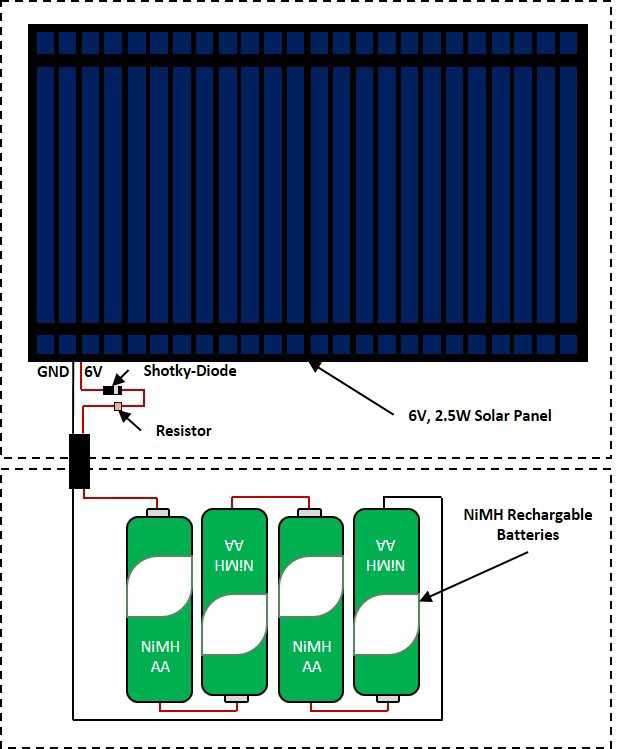
\includegraphics[keepaspectratio]{assets/PAR-solar-wiring.png}}

}

\caption{\label{fig-PAR_wiring}wiring scheme for the PAR sensor,
illustrating the electrical connections between the photodiode,
resistor, and microcontroller. The schematic focuses solely on the
wiring layout required for sensor assembly, not placement of additional,
non-electronical components within the sensor case.}

\end{figure}%

\subsubsection{Assembly Instructions:}\label{sec-solar-charger-assembly}

\begin{enumerate}
\def\labelenumi{\arabic{enumi}.}
\tightlist
\item
  Solder a 5cm black and red wire to + and -- pole of the solar panel.
\item
  Solder two 2x2 Screw terminal block (screw terminal 1 to 4) on the
  tiny perfboard/PCB board.
\item
  Remove 0,5cm isolation from the red wire coming from the solar panel
  and fix it in screw terminal 1.
\item
  Connect screw terminal 1 (Anode) and 2 (cathode) using the
  shotky-diode.
\item
  Connect screw terminal 2 and 3 using the 10 Ohm resistor.
\item
  Connect screw terminal 3 with + of the 4AA battery holder (using a red
  wire).
\item
  Remove 0,5cm isolation from the black wire coming from the solar panel
  and fix it in screw terminal 4.
\item
  Connect screw terminal 4 with - of the 4AA battery holder (using a
  black wire).
\item
  Seal solder connections using e.g.~transparent nail polish.
\end{enumerate}

\subsubsection{Calibration:}\label{sec-solar-charger-calibration}

Precise calibration is not required. To verify functionality, insert
fully discharged NiMH batteries of the same type and capacity into the
holder and expose the solar panel to direct sunlight for several hours.
A gradual voltage increase indicates proper trickle charging. A
current-limiting resistor (e.g., 10 Ω) is used to regulate charging
current, based on Ohm's Law (I = V / R). This ensures a safe, low
current suitable for trickle charging, typically around 1/100th of the
battery capacity per hour (e.g., 20 mA for 2000 mAh cells). The resistor
value can be adjusted to suit panel output and battery size---higher
resistance lowers the current to prevent overcharging in bright
sunlight.

\subsubsection{Code:}\label{sec-solar-charger-code}

No specific code is provided for this module, as it operates passively
without a microcontroller.

\subsection{Photosynthetic Active Radiation (PAR)
Sensor}\label{sec-par-sensor}

\subsubsection{Purpose \& Use Case:}\label{sec-par-sensor-purpose}

The PAR sensor module presented here can be used to determine
photosynthetically active radiation (PAR), the range of solar radiation
between 400 and 700 nm that is relevant for plant photosynthesis. While
this chapter focuses on the construction and calibration of the sensor
itself, it is designed to be integrated into larger monitoring setups
that include power supply and data logging via a microcontroller. The
sensor module thus serves as a \textbf{Component} in more comprehensive
systems---such as automatic climate stations or gas flux chambers
described in later chapters---where continuous PAR measurements are
essential for understanding environmental conditions and light-driven
plant processes.

\textbf{Bill of Materials:} \{\#sec-par-sensor-bom\}

A comprehensive overview of all components required to build the sensor,
needed quantities, recommended suppliers and approximate prices (in €)
is provided in Table~\ref{tbl-PAR_sensor_bom}.

\begin{longtable}[]{@{}
  >{\raggedright\arraybackslash}p{(\linewidth - 6\tabcolsep) * \real{0.2603}}
  >{\raggedright\arraybackslash}p{(\linewidth - 6\tabcolsep) * \real{0.2466}}
  >{\raggedright\arraybackslash}p{(\linewidth - 6\tabcolsep) * \real{0.2466}}
  >{\raggedright\arraybackslash}p{(\linewidth - 6\tabcolsep) * \real{0.2466}}@{}}
\caption{Components required for PAR sensor assembly; includes quantity,
typical suppliers, and approximate prices (no links provided due to
frequent changes).}\label{tbl-PAR_sensor_bom}\tabularnewline
\toprule\noalign{}
\begin{minipage}[b]{\linewidth}\raggedright
\textbf{Component}
\end{minipage} & \begin{minipage}[b]{\linewidth}\raggedright
\textbf{Amount}
\end{minipage} & \begin{minipage}[b]{\linewidth}\raggedright
\textbf{Supplier}
\end{minipage} & \begin{minipage}[b]{\linewidth}\raggedright
\textbf{Price (approx.)}
\end{minipage} \\
\midrule\noalign{}
\endfirsthead
\toprule\noalign{}
\begin{minipage}[b]{\linewidth}\raggedright
\textbf{Component}
\end{minipage} & \begin{minipage}[b]{\linewidth}\raggedright
\textbf{Amount}
\end{minipage} & \begin{minipage}[b]{\linewidth}\raggedright
\textbf{Supplier}
\end{minipage} & \begin{minipage}[b]{\linewidth}\raggedright
\textbf{Price (approx.)}
\end{minipage} \\
\midrule\noalign{}
\endhead
\bottomrule\noalign{}
\endlastfoot
Photodiode BPW34 & 1 & Amazon, Reichelt, Conrad & 0.70 € \\
Common E-Series electronic resistor (e.g., 2.2kΩ, 4.7kΩ or 10kΩ) & 1 &
Amazon, Reichelt, Conrad & 0.10 € \\
Visible light bandpass filter (400--700 nm; ⌀ 9.5 mm) & 1 & Aliexpress &
0.50 € \\
Polytetrafluoroethylene (PTFE) diffusor disk (⌀ 10 mm) & 1 & Amazon &
0.10 € \\
3D-printed PAR sensor case & 1 & -- & 0.10 € \\
3-wire cable, shielded, suitable for outdoor use (e.g., ⌀4 mm,
\textasciitilde1 m) & 1 & Amazon, Reichelt, Conrad & 0.50 € \\
\textbf{Sum} & & & \textbf{2.00 €} \\
\end{longtable}

\subsubsection{Wiring Diagram:}\label{sec-par-sensor-wiring}

A schematic overview of the wiring layout, showing all necessary
connections between electrical components, is provided in Figure
2.1.2.3.

\begin{figure}

\centering{

\pandocbounded{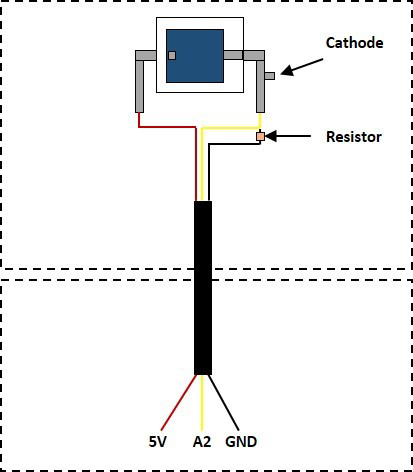
\includegraphics[keepaspectratio]{assets/PAR-sensor-wiring.png}}

}

\caption{\label{fig-PAR_sensor_wiring}Wiring scheme for the PAR sensor,
illustrating the electrical connections between the photodiode,
resistor, and microcontroller. The schematic focuses solely on the
wiring layout required for sensor assembly, not placement of additional,
non-electronical components within the sensor case.}

\end{figure}%

\subsubsection{Assembly Instructions:}\label{sec-par-sensor-assembly}

\begin{enumerate}
\def\labelenumi{\arabic{enumi}.}
\item
  3D-print case (black) using UV-resistant material
\item
  Place the BPW34 photodiode into the designated slot in the 3D-printed
  case, ensuring correct orientation (cathode/anode);
\item
  Solder 5V (red) and signal (e.g., A2) wire (yellow) of the cable to
  anode (horizontal mark on leg) and cathode of the BPW34, respectively;
\item
  Connect electrical resistor (no specific orientation) by solder one
  leg to the signal (e.g., A2) wire (yellow) and the other to GND wire
  (black) of the cable;
\item
  Seal solder connections using e.g.~transparent nail polish;
  Build-It-Yourself: Low-Cost Systems for Field Ecophysiology 10
\item
  Place the visible light bandpass filter over the BPW34 inside the
  3D-printed case;
\item
  Place the PTFE diffusor over the visible light bandpass filter and
  BPW34 on top of the 3D-printed case;
\item
  Seal 3D-printed case where necessary using e.g., silicon.
\item
  Connect the three-wire cable to the respective connections (5V, GND,
  signal (e.g., A2))
\item
  Upload program code to microcontroller and check if the sensor is
  delivering values in expected range under different light conditions;
\end{enumerate}

\subsubsection{Calibration:}\label{sec-par-sensor-calibration}

Since the sensor provides only an analog voltage output, it must be
calibrated to convert readings into meaningful units of
photosynthetically active radiation (PAR; μmol m⁻² s⁻¹). This requires
deriving a calibration function by operating the low-cost sensor
alongside a high-accuracy PAR sensor under natural sunlight over the
course of a clear day. Calibration is particularly important because
different resistor values can be used to adjust the sensor's sensitivity
to local light conditions. Lower resistor values reduce sensitivity,
making them suitable for high-light environments (e.g., inner
latitudes), while higher resistor values increase sensitivity but may
lead to signal saturation under intense light.
Section~\ref{sec-appendix_D} (Supporting Data) contains a 48h data set
of a low-cost PAR sensor directly compared with a high-cost SKP215 PAR
sensor (trueness; Campbell Scientific, UK) as well as a 36h test of 10
low-cost PAR sensors directly compared with a high-cost SKP215 PAR
sensor (accuracy; \textbf{Campbell Scientific, UK}).

\subsubsection{Code:}\label{sec-par-sensor-code}

Below, a basic Arduino IDE code example is given to implement the
low-cost DIY PAR sensor with a microcontroller (e.g., UNO, ProMini,
etc.).

\begin{Shaded}
\begin{Highlighting}[]
\CommentTok{// PAR sensor code}
\AttributeTok{const} \DataTypeTok{int}\NormalTok{ sensorPin }\OperatorTok{=}\NormalTok{ A0}\OperatorTok{;} \CommentTok{// Analog pin connected to photodiode anode}
\DataTypeTok{int}\NormalTok{ sensorValue }\OperatorTok{=} \DecValTok{0}\OperatorTok{;} \CommentTok{// Variable to store the raw analog value}
\DataTypeTok{void}\NormalTok{ setup}\OperatorTok{()} \OperatorTok{\{}
\NormalTok{Serial}\OperatorTok{.}\NormalTok{begin}\OperatorTok{(}\DecValTok{9600}\OperatorTok{);} \CommentTok{// Initialize serial communication}
\OperatorTok{\}}
\NormalTok{Build}\OperatorTok{{-}}\NormalTok{It}\OperatorTok{{-}}\NormalTok{Yourself}\OperatorTok{:}\NormalTok{ Low}\OperatorTok{{-}}\NormalTok{Cost Systems }\ControlFlowTok{for}\NormalTok{ Field Ecophysiology}
\DecValTok{11}
\DataTypeTok{void}\NormalTok{ loop}\OperatorTok{()} \OperatorTok{\{}
\NormalTok{sensorValue }\OperatorTok{=}\NormalTok{ analogRead}\OperatorTok{(}\NormalTok{sensorPin}\OperatorTok{);} \CommentTok{// Read analog value from sensor}
\NormalTok{Serial}\OperatorTok{.}\NormalTok{println}\OperatorTok{(}\NormalTok{sensorValue}\OperatorTok{);} \CommentTok{// Print value to serial monitor}
\NormalTok{delay}\OperatorTok{(}\DecValTok{1000}\OperatorTok{);} \CommentTok{// Wait for 1 second}
\OperatorTok{\}}
\end{Highlighting}
\end{Shaded}

\subsection{Environmental Variable Explorer (EVE
platform)}\label{sec-eve-platform}

\subsubsection{EVE-Offline Workflow (EVE platform; Weather station
config.)}\label{sec-eve-offline}

\paragraph{Purpose \& Use Case:}\label{sec-eve-offline-purpose}

EVE-Offline (Environmental Variable Explorer), configurated as a
compact, low-cost weather station designed for long-term monitoring of
environmental variables. It records PAR (400--700 nm), relative humidity
(RH), air temperature, and air pressure at a user-defined (e.g.,
30-minute interval). This setup enables continuous observation of
site-specific weather conditions throughout cropping seasons or even
across years. Data retrieval is realized via an Android application
(``MonksHillLab Logger App''). This chapter focuses on the construction,
calibration, and data retrieval. Continuous environmental data provided
by the system helps contextualize physiological responses and supports a
more accurate interpretation of crop--environment interactions.

\paragraph{Bill of Materials:}\label{sec-eve-offline-bom}

A comprehensive overview of all components required to build the
automatic weather station, needed quantities, recommended suppliers and
approximate prices (in €) is provided in Table~\ref{tbl-aws_bom}.

\begin{longtable}[]{@{}
  >{\raggedright\arraybackslash}p{(\linewidth - 6\tabcolsep) * \real{0.2603}}
  >{\raggedright\arraybackslash}p{(\linewidth - 6\tabcolsep) * \real{0.2466}}
  >{\raggedright\arraybackslash}p{(\linewidth - 6\tabcolsep) * \real{0.2466}}
  >{\raggedright\arraybackslash}p{(\linewidth - 6\tabcolsep) * \real{0.2466}}@{}}
\caption{Components required for weather station assembly; includes
quantity, typical suppliers, and approximate prices (no links provided
due to frequent changes).}\label{tbl-aws_bom}\tabularnewline
\toprule\noalign{}
\begin{minipage}[b]{\linewidth}\raggedright
\textbf{Component}
\end{minipage} & \begin{minipage}[b]{\linewidth}\raggedright
\textbf{Amount}
\end{minipage} & \begin{minipage}[b]{\linewidth}\raggedright
\textbf{Supplier}
\end{minipage} & \begin{minipage}[b]{\linewidth}\raggedright
\textbf{Price (approx.)}
\end{minipage} \\
\midrule\noalign{}
\endfirsthead
\toprule\noalign{}
\begin{minipage}[b]{\linewidth}\raggedright
\textbf{Component}
\end{minipage} & \begin{minipage}[b]{\linewidth}\raggedright
\textbf{Amount}
\end{minipage} & \begin{minipage}[b]{\linewidth}\raggedright
\textbf{Supplier}
\end{minipage} & \begin{minipage}[b]{\linewidth}\raggedright
\textbf{Price (approx.)}
\end{minipage} \\
\midrule\noalign{}
\endhead
\bottomrule\noalign{}
\endlastfoot
PAR sensor & 1 & DIY (see handbook) & 2.00 € \\
HC-05 / HC-06 Bluetooth Wireless RF Transceiver Module (RS232 TTL) & 1 &
AZ-Delivery, Amazon, Reichelt, Conrad & 3.50 € \\
Microcontroller (e.g., Pro Mini) & 1 & AZ-Delivery, Amazon & 3.50 € \\
TPL5110 Nano Power Timer & 1 & Antratek, BerryBase & 8.30 € \\
BMP280 (weatherproof) & 1 & Aliexpress & 3.50 € \\
RTC module (I2C; DS3231; 3.3V) & 1 & Amazon, BerryBase & 3.00 € \\
FRAM module (5V; 32kb) & 1 & Amazon, BerryBase, Aliexpress & 3.00 € \\
DC-DC step down converter & 1 & Amazon & 0.50 € \\
SHT40 module (weather proof) & 1 & Aliexpress & 4.70 € \\
3D-printed PAR sensor/SHT41 case (EVE) & 1 & - & 0.50 € \\
Weatherproof junction box (10.0×6.8×5.0 cm) & 1 & Amazon & 3.00 € \\
PG7 cable fitting & 2 & Hardware store & 0.50 € \\
4AA Battery holder & 1 & Amazon, Reichelt & 0.50 € \\
NiMH Battery (2300 mAh; rechargeable) & 4 & Amazon, Reichelt & 3.80 € \\
9V battery clip & 1 & Amazon & 0.10 € \\
Dupont connectors / headers / wires / terminal blocks & - & Amazon &
0.50 € \\
Perfboard / MonksHillLab PCB board (5×7 cm) & 1 & Amazon & 2.00 € \\
3-/4-wire cable, shielded (⌀4 mm, \textasciitilde10 cm, outdoor
suitable) & 1 & Amazon, Reichelt, Conrad & 0.50 € \\
\textbf{Sum} & & & \textbf{44.40 €} \\
\end{longtable}

\paragraph{Wiring Diagram:}\label{sec-eve-offline-wiring}

A schematic overview of the wiring layout, showing all necessary
connections between electrical components, is provided in
Figure~\ref{fig-EVE_wiring}.

\begin{figure}

\centering{

\pandocbounded{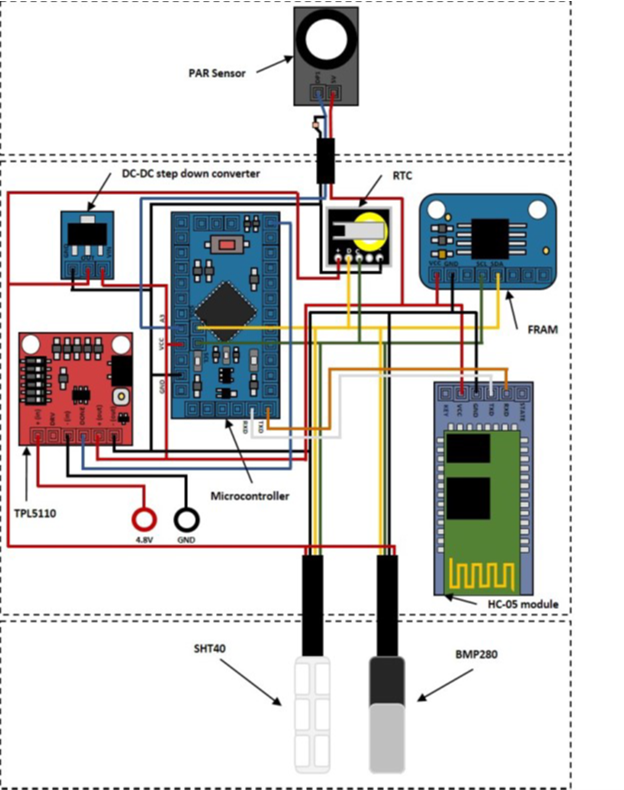
\includegraphics[keepaspectratio]{assets/EVE-wiring.png}}

}

\caption{\label{fig-EVE_wiring}Wiring scheme for the EVE-Offline weather
station configuration, illustrating the electrical connections between
the TPL5110, Pro Mini Microcontroller, DC-DC converter, FRAM and RTC
module as well as connected sensors (BMP280, SHT40 and PAR sensor). The
schematic focuses solely on the wiring layout required for weather
station assembly, not placement of additional, non-electronical
components within the outdoor case.}

\end{figure}%

\paragraph{Assembly Instructions:}\label{sec-eve-offline-assembly}

The following section provides a step-by-step assembly guide for
constructing the PAR sensor, detailing the integration of all
components: 1. 3D-print PAR sensor case (EVE; black) and SHT41 sensor
case (white) using UV-resistant material 2. Assemble PAR sensor as
explained within this handbook 3. Drill holes (Ø 4 mm) at the midpoint
of one vertical side (top) of the weatherproof junction box 4. Fit the
3-wire cable connected to the PAR sensor through one of these hole and
glue the PAR sensor on top of it 5. Fit PG7 on top of the 3D-printed
SHT40 case (smaller part), glue smaller part and larger part of
3D-printed SHT40 case on top of each other, fit SHT40 cable through it
until sensor head is fully covered by case and tighten PG7 up around the
4-wire cable of SHT40; finally fit 4-wire cable of SHT40 through one of
two Ø 10 mm holes drilled into the vertical side of the weatherproof
junction box, opposite to installed PAR sensor; fix wire to box with
PG7; fit BMP280 through the second hole and fix with 2nd PG7 6. Solder
female header (for electronical components) and screw terminal blocks
onto perfboard/PVB board as indicated (MonksHillLab PCB is suggested
cause easier to assemble) 7. Solder male header on bottom side of
electronical components 8. Fit electronical components with male header
on designated location with female header 9. Fix red and black wire of
9V battery clip in 2-Screw terminal block to GND (black) and 4.8V (red)
10. Fix red, black and blue wire of PAR sensor in 3-Screw terminal block
to GND (black), 5V (red) and A3 (blue) 11. Fix red, black, green and
yellow wire of SHT41 sensor in 4-Screw terminal block to GND (black), 5V
(red), SCL (green) and SDA (yellow) 12. In case perfboard and not PCB
board is used, connect components using color coded wires as indicated
in wiring scheme on perfboard 13. Crimp a male and female Dupont
connector to 4 7 cm wires (black, red, brown and white) and use these
wires to connect the HC-05 Bluetooth module with the microcontroller
through connecting VCC (red; HC-05) to VCC (red; microcontroller), GND
(black; HC-05) to GND (black; microcontroller), TX (white; HC-05) to RX
(white; microcontroller) and RX (brown; HC-05) to TX (brown;
microcontroller) 14. Fit (double sided tape) HC-05 Bluetooth module to
weatherproof junction box 15. Seal solder connections using
e.g.~transparent nail polish; 16. Upload program code to microcontroller
and check if the sensors are delivering values and if TPL5110 shuts the
system off/on as intended; 17. Connect to weather station using the
MonksHillLab App and test to dump data on mobile and reset FRAM

\paragraph{Calibration:}\label{sec-eve-offline-calibration}

The PAR sensor, which outputs analog voltage, requires calibration
against a high-accuracy PAR sensor under natural sunlight to derive a
conversion function to μmol m⁻² s⁻¹. Temperature, relative humidity, and
air pressure sensors do not require direct calibration but can be
validated by comparing readings with a reference-grade weather station.
Section~\ref{sec-appendix_D} (Supporting Data) contains a 48h data set
of a low-cost PAR sensor directly compared with a high-cost SKP215 PAR
sensor (trueness; Campbell Scientific, UK) as well as a 36h test of 10
low-cost PAR sensors directly compared with a high-cost SKP215 PAR
sensor (accuracy; Campbell Scientific, UK). In addition,
Section~\ref{sec-appendix_D} (Supporting Data) contains a 7 days field
deployment test/proof of concept of EVE-Offline, comparing air
temperature and RH readings with high-cost instruments.

\paragraph{Code:}\label{sec-eve-offline-code}

Please see Arduino IDE code example given in
Section~\ref{sec-appendix_A} to implement the offline workflow of the
automatic weather station configuration of EVE. The required Android
Application (``MonksHillLab Logger App'') can be found in
Section~\ref{sec-appendix_C}.

\paragraph{Backend infrastructure and dashboard
setup:}\label{sec-eve-offline-backend}

Operation of the EVE-Online weather station configuration does not
require programming expertise, but it does require access to a basic web
server environment supporting PHP and MySQL. This can be provided by
institutional infrastructure (e.g., a university server), a
low-cost/free of charge shared web hosting service, or a local
installation using a standard web server stack (e.g., XAMPP). The
backend consists of a lightweight database and web dashboard that manage
users, measurement sites, sensor nodes, and incoming data streams.
Initial setup involves creating an empty MySQL database and importing a
predefined SQL schema (provided in the Section~\ref{sec-appendix_C}).
Executing this schema automatically generates all required tables for
user management, site configuration, node registration, and sensor data
storage. The dashboard code is supplied as a ready-to-use package
(Section~\ref{sec-appendix_C}) and deployed by copying the contents of
the provided www directory into the web server's document root (e.g.,
public\_html or www). Configuration files allow users to specify
database credentials and define a secure authentication token that links
individual EVE nodes to the backend. Once configured, a single
initialization script is executed to create an administrator account.
After setup, users can access the web-based dashboard to register
measurement sites, assign sensor nodes, monitor incoming data in
near--real time, and download datasets for further analysis. This
backend design deliberately avoids complex dependencies and proprietary
services, providing a transparent, self-hosted data pipeline that
remains fully under user control.

\section{Plant Responses}\label{sec-plant-responses}

\subsection{Handheld System to measure Spectral Plant Indices (e.g.,
NDVI, PRI)}\label{sec-handheld-spectral}

\subsubsection{Purpose \& Use
Case:}\label{sec-handheld-spectral-purpose}

The handheld spectral measurement system presented here enables
low-cost, in-situ measurement of vegetation indices by capturing
reflectance data across six distinct wavelengths in the visible and/or
near-infrared (NIR) wavelengths. These spectral measurements allow the
calculation of widely used indices such as the Normalized Difference
Vegetation Index (NDVI) and the Photochemical Reflectance Index (PRI),
providing insights into plant physiological or health status, canopy
structure, and light-use efficiency. This chapter focuses on the
construction, calibration, and application of the handheld system tio
measure spectral plant indices, which is designed for flexible
deployment in field experiments, precision agriculture, and ecological
monitoring. While primarily intended as a standalone handheld system,
the working principle of made measurements can also be integrated into
automatic systems.

\subsubsection{Bill of Materials:}\label{sec-handheld-spectral-bom}

A comprehensive overview of all components required to build the
handheld measurement system for spectral plant indices, needed
quantities, recommended suppliers and approximate prices (in €) is
provided in Table~\ref{tbl-spectral_indices_bom}.

\begin{longtable}[]{@{}
  >{\raggedright\arraybackslash}p{(\linewidth - 6\tabcolsep) * \real{0.2703}}
  >{\raggedright\arraybackslash}p{(\linewidth - 6\tabcolsep) * \real{0.2432}}
  >{\raggedright\arraybackslash}p{(\linewidth - 6\tabcolsep) * \real{0.2432}}
  >{\raggedright\arraybackslash}p{(\linewidth - 6\tabcolsep) * \real{0.2432}}@{}}
\caption{Components required for assembly of the handheld system to
measure spectral plant indices; includes quantity, typical suppliers,
and approximate prices (no links provided due to frequent
changes).}\label{tbl-spectral_indices_bom}\tabularnewline
\toprule\noalign{}
\begin{minipage}[b]{\linewidth}\raggedright
\textbf{Component}
\end{minipage} & \begin{minipage}[b]{\linewidth}\raggedright
\textbf{Amount}
\end{minipage} & \begin{minipage}[b]{\linewidth}\raggedright
\textbf{Supplier}
\end{minipage} & \begin{minipage}[b]{\linewidth}\raggedright
\textbf{Price (approx.)}
\end{minipage} \\
\midrule\noalign{}
\endfirsthead
\toprule\noalign{}
\begin{minipage}[b]{\linewidth}\raggedright
\textbf{Component}
\end{minipage} & \begin{minipage}[b]{\linewidth}\raggedright
\textbf{Amount}
\end{minipage} & \begin{minipage}[b]{\linewidth}\raggedright
\textbf{Supplier}
\end{minipage} & \begin{minipage}[b]{\linewidth}\raggedright
\textbf{Price (approx.)}
\end{minipage} \\
\midrule\noalign{}
\endhead
\bottomrule\noalign{}
\endlastfoot
Microcontroller (e.g., UNO) & 1 & AZ-Delivery, Amazon, Reichelt, Conrad
& 9.00 € \\
HC-05 / HC-06 Bluetooth Wireless RF Transceiver Module (RS232 TTL) & 1 &
AZ-Delivery, Amazon, Reichelt, Conrad & 9.00 € \\
AS7262/AS7263 6-channel spectral sensor & 2 & Aliexpress, Antratek,
BerryBase & 60.00 € \\
TCA9548A I2C Multiplexer & 1 & AZ-Delivery, Amazon, Reichelt, Conrad &
3.00 € \\
PTFE diffuser disk (⌀ 40 mm) & 1 & Amazon & 0.50 € \\
3D-printed AS7262/AS7263 sensor case & 2 & - & 1.00 € \\
3D-printed TCA9548A case & 1 & - & 0.50 € \\
Rocker switch (round) & 1 & Amazon & 1.00 € \\
HMF ODK500 Outdoor case (19×13×5.5 mm) & 1 & Amazon & 20.00 € \\
6×AA battery holder & 1 & Amazon & 2.00 € \\
NiMH batteries (2300 mAh, rechargeable) & 6 & Amazon, Reichelt, Conrad &
14.00 € \\
9V battery clip & 1 & Amazon & 0.50 € \\
4-wire USB-A extension cable (\textasciitilde1 m, shielded, outdoor) & 1
& Amazon, Reichelt, Conrad & 3.50 € \\
Dupont connectors (female) / terminal blocks & 4 & Amazon & 1.00 € \\
Wires (black, red, yellow, green, blue, brown) & - & Amazon & 0.50 € \\
Aluminum/steel rods, wood or PVC pipe (4 m) & 1 & Hardware store & 20.00
€ \\
\textbf{Sum} & & & \textbf{145.50 €} \\
\end{longtable}

\subsubsection{Wiring Diagram:}\label{sec-handheld-spectral-wiring}

A schematic overview of the wiring layout, showing all necessary
connections between electrical components, is provided in
Figure~\ref{fig-spectral_indices_wiring}.

\begin{figure}

\centering{

\pandocbounded{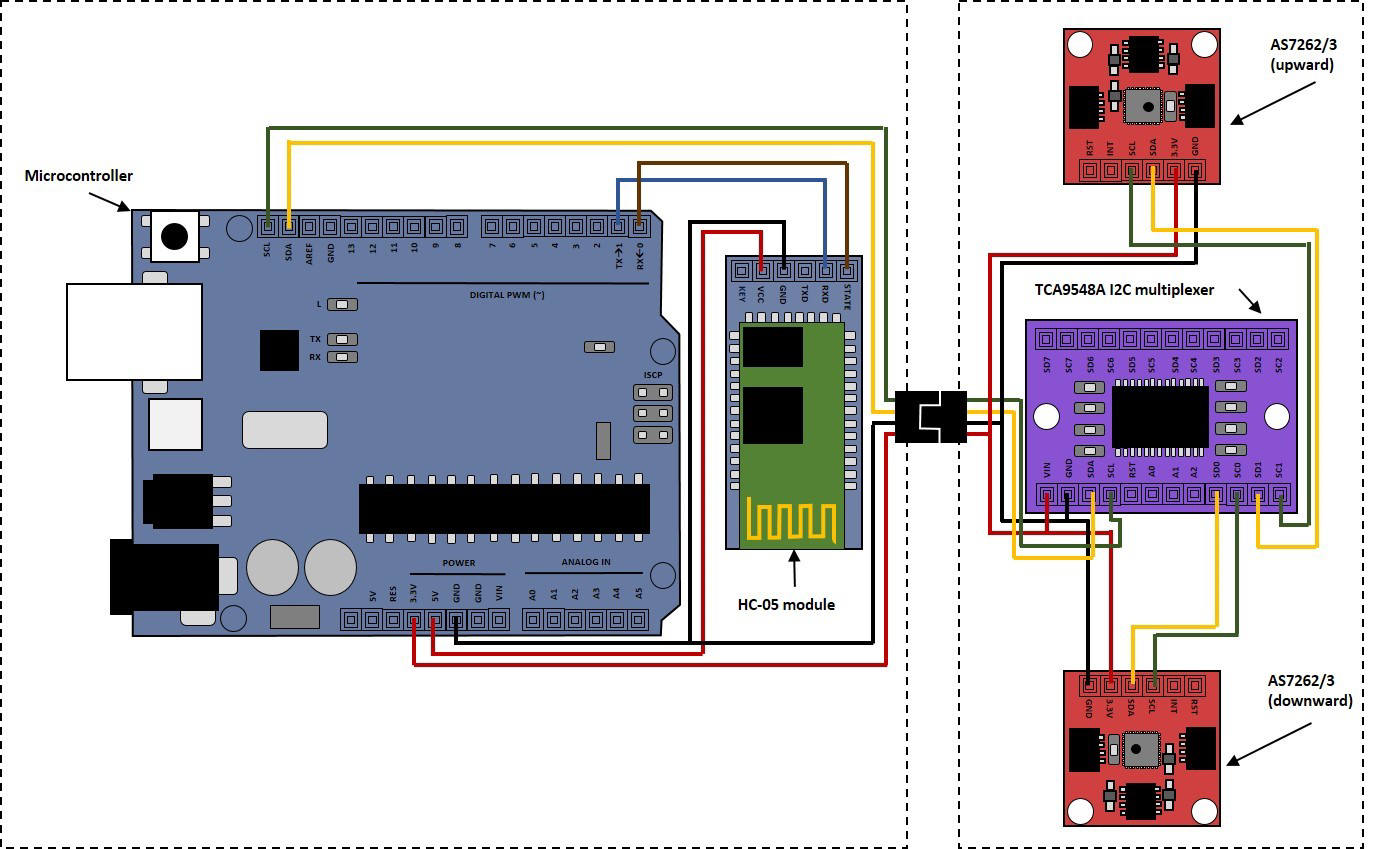
\includegraphics[keepaspectratio]{assets/spectral-plant-indices-wiring.png}}

}

\caption{\label{fig-spectral_indices_wiring}Wiring scheme for the
handheld system to measure Spectral Plant Indices, illustrating the
electrical connections between the spectral sensors, I2C multiplexer,
Bluetooth module and microcontroller. The schematic focuses solely on
the wiring layout required for system assembly, not placement of
additional, non-electronical components within the sensor and/or battery
case.}

\end{figure}%

\subsubsection{Assembly
Instructions:}\label{sec-handheld-spectral-assembly}

The following section provides a step-by-step assembly guide for
constructing the handheld system to measure spectral plant indices,
detailing the integration of all components: 1. 3D-print cases (black)
using UV-resistant material; 2. Solder 5cm long wires to 3.3V (red), GND
(black), SCL (green) and SDA (yellow) of one of the AS7262/3 and fix
(glue or double sided tape) it to 3D-printed AS7262/3 case (upward
case/smaller outer walls); fit loose ends through its back 3. Fix
(double sided tape) TCA9548A I2C multiplexer to the back of the upward
case 4. Fix (double sided tape) 6-Luster clamp to top of TCA9548A I2C
multiplexer 5. Solder loose ends of the 5cm long wire for SCL (green)
and SDA (yellow) to SC0 (green) and SD0 (yellow) of TCA9548A I2C
multiplexer; 6. Fix loose ends of 5cm long wires for 3.3V (red) and GND
(black) to 1 and 2 of the 6-luster clamp 7. Solder 15cm (!) long 3.3V
(red), GND (black), SCL (green) and SDA (yellow) to the second of the
AS7262/3 and fix (glue or double sided tape) it to 3D-printed AS7262/3
case (downward case/taller outer walls); fit loose ends through its back
8. Solder 5cm long wires for 3.3V (red), GND (black), SCL (green) and
SDA (yellow) to VIN (red), GND (black), SCL (green) and SDA (yellow) of
TCA9548A and fix their loose ends to 6-luster clamp 1, 2, 3 and 4 9.
Solder 5cm long wires for SCL (green) and SDA (yellow) to SC1 (green)
and SD1 (yellow) of TCA9548A and fix their loose ends to luster clamp 5
and 6 10. Fix loose ends of 15cm long wires for 3.3V (red), GND (black),
SCL (green) and SDA (yellow) to 1, 2 5 and 6 of the 6-luster clamp 11.
Cut 4-wire USB A extension cable into two similar long parts and remove
ca. 5cm isolation on loose ends; fit one loose end through the hole in
the TCA9548A case and connect the red, black, green and yellow wire of
the USB A cable to luster clamp 1, 2, 3 and 4 (in case of different
colors in USB A cable allocate wire color) 12. Drill a 5mm hole into the
top end of the HMF ODK500 Outdoor case and a 20mm hole into the cover
flap positioned near the hinge to insert the second USB A cable and
install the rocker switch 13. Solder the red, black, green and yellow
wire of the USB A cable to 3.3V, GND, SCL and SDA of the microcontroller
14. Solder 9V battery clip red wire to one of the rocker switch
connectors and solder a 10cm long red wire to its second contact; than
solder black wire of 9V battery clip and loose end of 10cm red wire to
GND and VIN of microcontroller 15. Fix microcontroller to the box using
e.g.~double sided tape and insert batteries into 6AA battery holder and
place it into the box as well (fix if necessary) 16. Solder a 7cm long
red, black, white and blue cable to 5V, GND, TX and RX of the
microcontroller and crimp a female Dupont connector to the loose wire
ends; 17. Connect Dupont connectors on 5V, GND, TX and RX wires from
microcontroller to VCC, GND, RX and TX male pins at HC-05 Bluetooth
module and place the module within the box (note: RX goes to TX and TX
to RX) 18. Seal solder connections using e.g.~transparent nail polish;
19. Place the PTFE diffusor over the upward directed AS7262/3 on top of
the 3D-printed case and connect cases together to form sensor head 20.
Seal 3D-printed sensor head where necessary using e.g., silicon. 21.
Construct a 1.8-meter high pole with a 1-meter long reinforced
cantilever arm and fix sensor head on arm using e.g., cable tie (make
sure sensors are directed up- and downwards as intended); fix
battery/microcontroller box on pole and connect USB A plug
(battery/microcontroller box) with socket (sensor head) 22. Upload
program code to microcontroller and check if the sensor is delivering
e.g., NDVI values in expected range via Bluetooth connection for
different surfaces/canopies using the MonksHillLab Logger App;

\subsubsection{Calibration:}\label{sec-handheld-spectral-calibration}

Since the sensor provides direct NDVI measurements based on reflectance
in selected spectral bands, measurement values does not need to be
converted prior to use. However, calibration is essential to ensure
accuracy and comparability across different setups and conditions. NDVI
values can be easily calibrated against reference surfaces with known
NDVI values to derive a correction function. A practical and low-cost
approach involves using colored reference targets, such as cardboards
with defined reflectance properties (e.g.~white, black, green, yellow),
as demonstrated by (Macagga et al. 2025).

\subsubsection{Code:}\label{sec-handheld-spectral-code}

Below, an Arduino IDE code example is given to implement the low-cost
DIY handheld NDVI measurement system.

\begin{verbatim}
// Handheld NDVI sensor code
#include <Wire.h>
#include <SPI.h>
#include "AS726X.h"
#include <SoftwareSerial.h>
#define AS7263_I2C_ADDRESS 0x49 // Default I2C address of AS7263
#define TCA_I2C_ADDRESS 0x70 // Address of the TCA9548A multiplexer
#define NUMBER_OF_SENSORS 2
#define DONEPIN 9 // Optional: for signaling when a cycle is done
AS726X accel; // Shared AS726X object for both sensors
// Variables
int cycles = 0;
float up_ir;
float up_vis;
float down_ir;
float down_vis;
float NDVI;
float NIRup;
float VISup;
float NIRdown;
float VISdown;
void setup() {
delay(1500);
Wire.begin();
Serial.begin(9600);
delay(1500);
// Initialize both AS726X sensors via TCA channels
setTCAChannel(0);
accel.begin(); // Initialize sensor on channel 0
delay(1500);
setTCAChannel(1);
accel.begin(); // Initialize sensor on channel 1
delay(1500);
}
void loop() {
// --- Top Sensor (Channel 0) ---
setTCAChannel(0);
accel.takeMeasurements();
up_ir = accel.getCalibratedS(); // Placeholder for IR reading (if needed)
VISup = accel.getCalibratedS(); // Get visible spectrum value
NIRup = accel.getCalibratedU() + accel.getCalibratedV(); // Combine NIR bands
Serial.print(VISup);
Serial.print(";");
Serial.print(NIRup);
delay(1500);
// --- Bottom Sensor (Channel 1) ---
setTCAChannel(1);
accel.takeMeasurements();
down_ir = accel.getCalibratedS(); // Placeholder
VISdown = accel.getCalibratedS(); // Get visible spectrum value
NIRdown = accel.getCalibratedU() + accel.getCalibratedV(); // Combine NIR bands
// NDVI Calculation
NDVI = ((NIRdown / NIRup) - (VISdown / VISup)) /
((NIRdown / NIRup) + (VISdown / VISup));
// Output data
Serial.print(";");
Serial.print(NDVI);
Serial.print(";");
Serial.print(VISdown);
Serial.print(";");
Serial.println(NIRdown);
delay(900);
}
// Selects the I2C channel on the TCA9548A multiplexer
void setTCAChannel(byte i) {
Wire.beginTransmission(TCA_I2C_ADDRESS);
Wire.write(1 << i);
Wire.endTransmission();
}
\end{verbatim}

\subsection{Automatic System to measure Spectral Plant Indices (e.g.,
NDVI, PRI)}\label{sec-automatic-spectral}

\subsubsection{Purpose \& Use
Case:}\label{sec-automatic-spectral-purpose}

The automatic system presented here enables automated monitoring of
spectral plant indices such as the NDVI and PRI, which are indicators of
plant health and photosynthetic activity. Unlike the handheld version
\textbf{(chapter 3)}, this system is designed for permanent installation
in the field and operates autonomously, recording data at regular
intervals---typically once per hour for e.g., 30 seconds---over extended
periods (weeks). This makes the system a valuable component for
long-term ecological studies, crop monitoring, or integration into
automated infrastructure such as stationary gas flux chambers or field
phenotyping platforms, where continuous, high-temporal-resolution NDVI
and PRI measurements are critical for analyzing plant responses to
environmental conditions.

\paragraph{Bill of Materials:}\label{sec-automatic-spectral-bom}

A comprehensive overview of all components required to build the
automatic measurement system for spectral plant indices, needed
quantities, recommended suppliers and approximate prices (in €) is
provided in Table~\ref{tbl-automatic_spectral_indices_bom}.

\begin{longtable}[]{@{}
  >{\raggedright\arraybackslash}p{(\linewidth - 6\tabcolsep) * \real{0.2917}}
  >{\raggedright\arraybackslash}p{(\linewidth - 6\tabcolsep) * \real{0.2361}}
  >{\raggedright\arraybackslash}p{(\linewidth - 6\tabcolsep) * \real{0.2361}}
  >{\raggedright\arraybackslash}p{(\linewidth - 6\tabcolsep) * \real{0.2361}}@{}}
\caption{Components required for assembly of the automatic system to
measure spectral plant indices; includes quantity, typical suppliers,
and approximate prices (no links provided due to frequent
changes).}\label{tbl-automatic_spectral_indices_bom}\tabularnewline
\toprule\noalign{}
\begin{minipage}[b]{\linewidth}\raggedright
Component
\end{minipage} & \begin{minipage}[b]{\linewidth}\raggedright
Qty
\end{minipage} & \begin{minipage}[b]{\linewidth}\raggedright
Supplier
\end{minipage} & \begin{minipage}[b]{\linewidth}\raggedright
Price
\end{minipage} \\
\midrule\noalign{}
\endfirsthead
\toprule\noalign{}
\begin{minipage}[b]{\linewidth}\raggedright
Component
\end{minipage} & \begin{minipage}[b]{\linewidth}\raggedright
Qty
\end{minipage} & \begin{minipage}[b]{\linewidth}\raggedright
Supplier
\end{minipage} & \begin{minipage}[b]{\linewidth}\raggedright
Price
\end{minipage} \\
\midrule\noalign{}
\endhead
\bottomrule\noalign{}
\endlastfoot
Microcontroller (e.g., Pro Mini) & 1 & AZ-Delivery, Amazon & 8.00 € \\
TPL5110 Nano Power Timer & 1 & Antratek, BerryBase & 8.00 € \\
AS7262/AS7263 6-channel spectral sensor & 2 & Aliexpress, Antratek,
BerryBase & 60.00 € \\
RTC module (I2C; DS3231; 3.3V) & 1 & Amazon, BerryBase & 5.00 € \\
TF Micro-SD-card module (3.3V) & 1 & Amazon & 2.00 € \\
DC-DC step-down converter & 1 & Amazon & 0.60 € \\
Micro-SD-card (16 GB) & 1 & Amazon & 6.00 € \\
TCA9548A I2C Multiplexer & 1 & AZ-Delivery, Amazon, Reichelt, Conrad &
3.00 € \\
PTFE diffusor disk (⌀ 40mm) & 1 & Amazon & 0.50 € \\
3D-printed AS7263/AS7262 sensor case & 2 & - & 1.00 € \\
3D-printed system case & 1 & - & 2.50 € \\
TFA Dostmann protective case & 1 & Amazon & 13.00 € \\
4AA Battery holder & 1 & Amazon & 2.00 € \\
NiMH Battery (2300 mAh; rechargeable) & 4 & Amazon, Reichelt, Conrad &
10.00 € \\
9V battery clip & 1 & Amazon & 0.50 € \\
Dupont connector (female) / luster clamps & 4 & Amazon & 1.00 € \\
Perfboard / MonksHillLab PCB board (5x7cm) & 1 & Amazon & 1.00 € \\
Wires (black, red, yellow, green, blue, brown) & - & Amazon & 0.50 € \\
Aluminum, steel rods, wood or PVC pipe (4m) & 1 & Hardware store & 20.00
€ \\
\textbf{Total} & & & \textbf{144.60 €} \\
\end{longtable}

\subsubsection{Wiring Diagram:}\label{sec-automatic-spectral-wiring}

A schematic overview of the wiring layout, showing all necessary
connections between electrical components, is provided in
Figure~\ref{fig-automatic_spectral_indices_wiring}.

\begin{figure}

\centering{

\pandocbounded{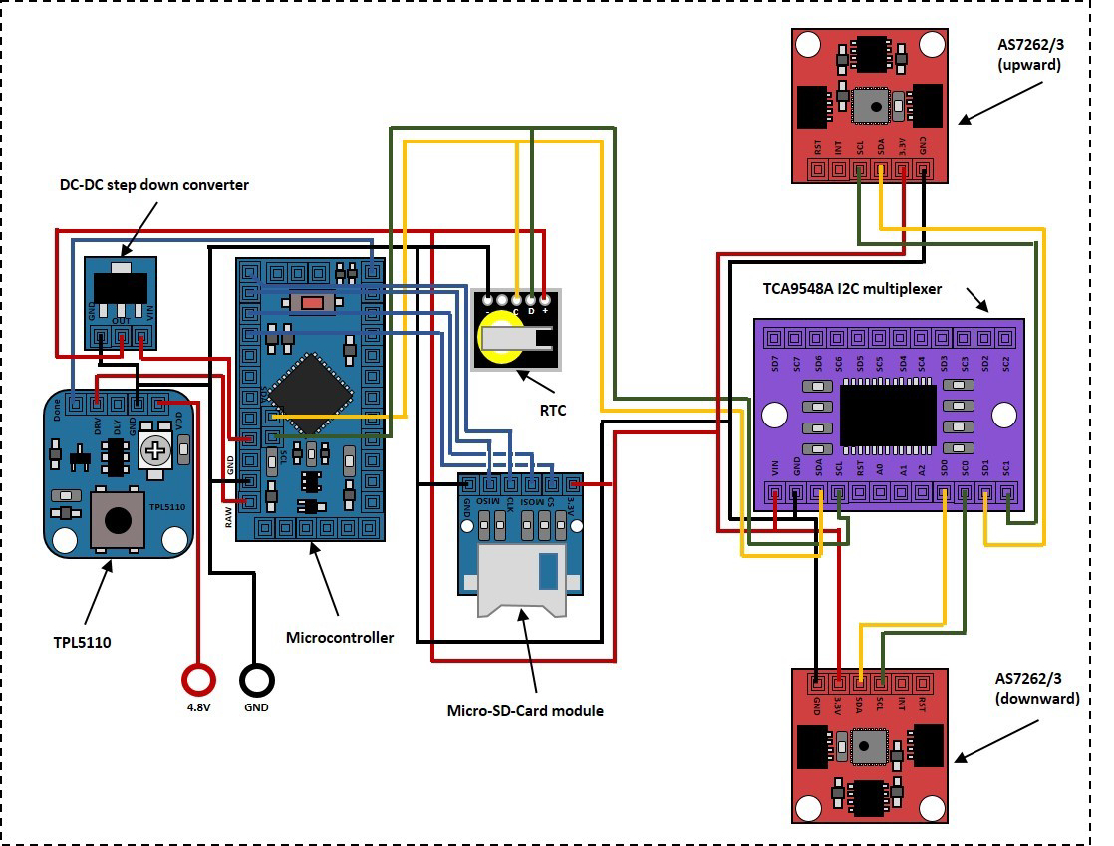
\includegraphics[keepaspectratio]{assets/automatic-spectral-plant-indices-wiring.png}}

}

\caption{\label{fig-automatic_spectral_indices_wiring}wiring scheme for
the automatic system to measure spectral plant indices, illustrating the
electrical connections between the spectral sensors, I2C multiplexer,
TPL5110, DC-DC step down converter, RTC module, Micro-SD-card module and
microcontroller. The schematic focuses solely on the wiring layout
required for system assembly, not placement of additional,
non-electronical components within the sensor and/or battery case.}

\end{figure}%

\subsubsection{Assembly
Instructions:}\label{sec-automatic-spectral-assembly}

The following section provides a step-by-step assembly guide for
constructing the automatic system to measure spectral plant indices,
detailing the integration of all components: 1. 3D-print cases (black)
using UV-resistant material; 2. Solder 15cm long wires to 3.3V (red),
GND (black), SCL (green) and SDA (yellow) of each of the AS7262/3 and
fix (glue or double sided tape) both to the 3D-printed AS7262/3 cases;
fit loose ends through its back and solder them to the top/bottom of the
PCB/perfboard; 3. Solder TPL5110 and microcontroller (e.g., Pro Mini) to
PCB/perfboard by connecting DRV (red; TPL5110) with RAW (red; Pro Mini),
Done (blue; TPL5110) with digital pin 9 (blue; Pro Mini) and GND (black;
TPL5110) with GND(black; Pro Mini) through wires and predrilled holes;
4. Solder DC-DC step down converter to PCB/perfboard by connecting VIN
(red; DC-DC) with VCC (red; Pro Mini), GND (black; DC-DC) with GND
(black; Pro Mini) and OUT (red; DC-DC) with 3.3V (red; AS7262/3) at the
top and bottom of PCB/perfboard through wires and predrilled holes; 5.
Connect GND (black) wireline with GND (black) coming from AS7262/3 at
the top and bottom of PCB/perfboard through wires; 6. Solder TCA9548A
I2C multiplexer to PCB/perfboard by connecting VIN (red; TCA9548A) with
3.3V (red; DC-DC), GND (black; TCA9548A) with GND (black; DC-DC), SDA
(yellow; TCA9548A) with A4 (yellow; Pro Mini) and SCL (green; TCA9548A)
with A5 (green; Pro Mini) through wires and predrilled holes; 7. Solder
RTC module to PCB/perfboard by connecting + (red; RTC) with 3.3V (red;
DC-DC), GND (black; RTC) with GND (black; DC-DC), SDA (yellow; RTC) with
A4 (yellow; Pro Mini) and SCL (green; RTC) with A5 (green; Pro Mini)
through wires and predrilled holes; 8. Solder Micro-SD-card module to
PCB/perfboard by connecting + (red; Micro-SD) with 3.3V (red; DC-DC),
GND (black; Micro-SD) with GND (black; DC-DC), CLK (blue; Micro-SD) with
digital pin 10 (blue; Pro Mini), MISO (blue; Micro-SD) with digital pin
11 (blue; Pro Mini), MOSI (blue; Micro-SD) with digital pin 12 (blue;
Pro Mini), CS (blue; Micro-SD) with digital pin 13 (blue; Pro Mini)
through wires and predrilled holes; 9. Connect SDA (yellow) and SCL
(green) from upward AS7262/3 to SD0 (yellow; TCA9548A) and SC0 (green;
TCA9548A) 10. Connect SDA (yellow) and SCL (green) from downward
AS7262/3 to SD1 (yellow; TCA9548A) and SC1 (green; TCA9548A) 11. Solder
4.8V (red) and GND (black) wire of the 9V battery clip to the TPL5110
VDD (red) and GND (black) ; 12. Fit PCB/perfboard and 4AA battery holder
with NiMh rechargeable batteries inside the system case and close case
with upward/downward sensor case; 13. Drill a Ø40mm hole into the middle
of the top and bottom of the TFA Dostmann climate station case; 14. Fix
(glue) the PTFE diffusor over the upward directed AS7262/3 on top of the
TFA Dostmann climate station case 15. Seal 3D-printed sensor head where
necessary using e.g., silicon. 16. Upload program code to
microcontroller and check if the sensor is storing e.g., NDVI values in
expected range on the micro-SD-card; 17. Construct a 1.8-meter high pole
with a 1-meter long reinforced cantilever arm and fix sensor head on arm
using e.g., cable tie (make sure sensors are directed up- and downwards
as intended);

\subsubsection{Calibration:}\label{sec-automatic-spectral-calibration}

Since the sensor provides direct NDVI measurements based on reflectance
in selected spectral bands, measurement values does not need to be
converted prior to use. However, calibration is essential to ensure
accuracy and comparability across different setups and conditions. NDVI
values can be easily calibrated against reference surfaces with known
NDVI values to derive a correction function. A practical and low-cost
approach involves using colored reference targets, such as cardboards
with defined reflectance properties (e.g.~white, black, green, yellow),
as demonstrated by Macagga et al. (2025).

\subsubsection{Code:}\label{sec-automatic-spectral-code}

Please see Arduino IDE code example given in
Section~\ref{sec-appendix_A} to implement the automatic low-cost DIY
NDVI measurement system.

\section{Biogeochemical Cycling}\label{sec-biogeochemical-cycling}

\subsection{Manual System to measure CO2 and ET
fluxes}\label{sec-manual-flux}

\subsubsection{Purpose \& Use Case:}\label{sec-manual-flux-purpose}

The sensor unit and data logger presented here can be used to determine
CO₂ and ET fluxes using the manual closed-chamber method---two key
fluxes in the C and water cycles, respectively. While this chapter
focuses on the construction, calibration, and deployment of the manual
version of the system, the setup is designed with flexibility in mind
and can be readily adapted for automated operation. This modularity
allows it to serve as a foundational component in both short-term field
campaigns and long-term environmental monitoring efforts. The data
generated provide critical insights into plant--soil--atmosphere
interactions, especially in relation to photosynthetic activity,
respiration, and water use. In later chapters, integration into
automated systems is explained to facilitate high-resolution, continuous
flux measurements across spatial and temporal scales.

\subsubsection{Bill of Materials:}\label{sec-manual-flux-bom}

A comprehensive overview of all components required to build the manual
system to measure CO2 and ET fluxes (excluding the closed-chamber),
needed quantities, recommended suppliers and approximate prices (in €)
is provided in Table~\ref{tbl-manual_flux_bom}.

\begin{longtable}[]{@{}
  >{\raggedright\arraybackslash}p{(\linewidth - 6\tabcolsep) * \real{0.2917}}
  >{\raggedright\arraybackslash}p{(\linewidth - 6\tabcolsep) * \real{0.2361}}
  >{\raggedright\arraybackslash}p{(\linewidth - 6\tabcolsep) * \real{0.2361}}
  >{\raggedright\arraybackslash}p{(\linewidth - 6\tabcolsep) * \real{0.2361}}@{}}
\caption{Components required for data logger and sensor unit assembly;
includes quantity, typical suppliers, and approximate prices (no links
provided due to frequent
changes).}\label{tbl-manual_flux_bom}\tabularnewline
\toprule\noalign{}
\begin{minipage}[b]{\linewidth}\raggedright
Component
\end{minipage} & \begin{minipage}[b]{\linewidth}\raggedright
Amount
\end{minipage} & \begin{minipage}[b]{\linewidth}\raggedright
Supplier
\end{minipage} & \begin{minipage}[b]{\linewidth}\raggedright
Price (approx.)
\end{minipage} \\
\midrule\noalign{}
\endfirsthead
\toprule\noalign{}
\begin{minipage}[b]{\linewidth}\raggedright
Component
\end{minipage} & \begin{minipage}[b]{\linewidth}\raggedright
Amount
\end{minipage} & \begin{minipage}[b]{\linewidth}\raggedright
Supplier
\end{minipage} & \begin{minipage}[b]{\linewidth}\raggedright
Price (approx.)
\end{minipage} \\
\midrule\noalign{}
\endhead
\bottomrule\noalign{}
\endlastfoot
Microcontroller (e.g., UNO) & 1 & AZ-Delivery, Amazon & 9.00 € \\
BMP280 & 1 & AZ-Delivery, Amazon & 2.00 € \\
K30 FR NDIR CO2 sensor & 1 & Driesen \& Kern & 80.00 € \\
Data logger shield (UNO) & 1 & AZ-Delivery, Amazon & 6.00 € \\
SHT41 module (weather proof) & 1 & Aliexpress & 8.00 € \\
HC-05 / HC-06 Bluetooth RF Transceiver Module (RS232 TTL) & 1 &
AZ-Delivery, Amazon, Reichelt, Conrad & 9.00 € \\
SD-card (2 GB) & 1 & Amazon & 5.00 € \\
0.96'' OLED display (I2C) & 1 & Amazon, AZ-Delivery & 5.00 € \\
PAR sensor & 1 & DIY (see handbook) & 3.45 € \\
3D-printed K30 FR sensor case & 1 & - & 1.00 € \\
B\&W Outdoor Case Typ 500 (yellow) & 1 & Profikoffer & 30.00 € \\
6AA Battery holder & 2 & Amazon & 4.00 € \\
NiMH Battery (2300 mAh; rechargeable) & 12 & Amazon, Reichelt, Conrad &
28.00 € \\
9V battery clip & 2 & Amazon & 1.00 € \\
Dupont connector (male/female) / luster clamps & 24 & Amazon & 6.00 € \\
Perfboard / MonksHillLab PCB board (5x7cm) & 1 & Amazon & 2.00 € \\
Wires / screw terminal blocks (various colors) & - & Amazon & 5.00 € \\
\textgreater10-wire cable, shielded (\textasciitilde1.5 m, outdoor
suitable) & 1 & Amazon & 8.00 € \\
Rocker switch (4 connections) & 1 & Amazon & 5.00 € \\
PG9 cable fitting & 1 & Hardware store & 2.00 € \\
Hard foam plate & 1 & Amazon & 5.00 € \\
\textbf{Total} & & & \textbf{224.50 €} \\
\end{longtable}

\subsubsection{Wiring Diagram:}\label{sec-manual-flux-wiring}

A schematic overview of the wiring layout, showing all necessary
connections between electrical components, is provided in
Figure~\ref{fig-manual_flux_system_wiring}.

\begin{figure}

\centering{

\pandocbounded{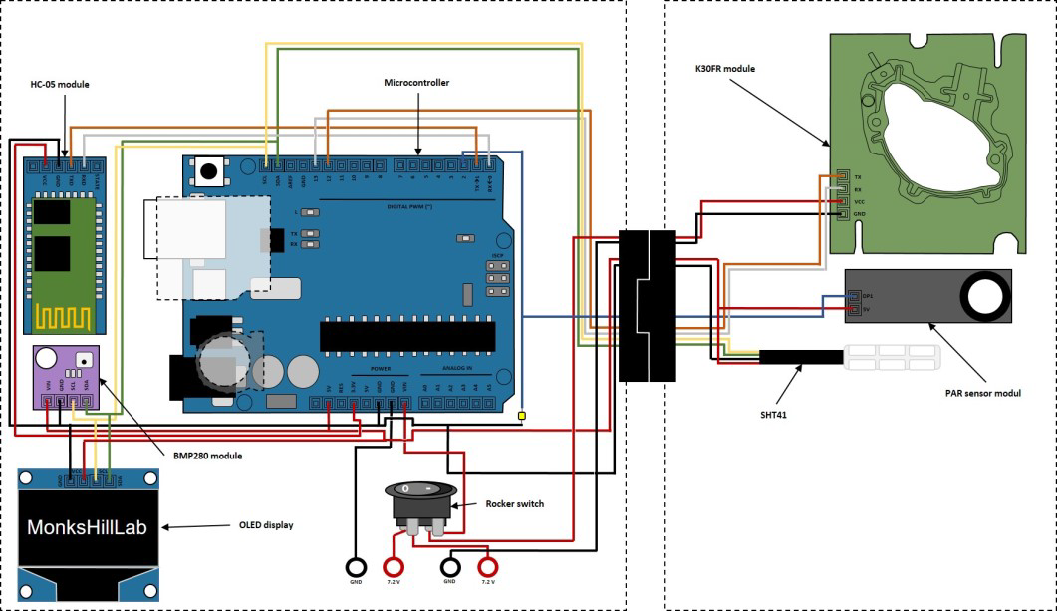
\includegraphics[keepaspectratio]{assets/manual-flux-system-wiring.png}}

}

\caption{\label{fig-manual_flux_system_wiring}Wiring scheme for the
manual system to measure CO2 and ET fluxes, illustrating the electrical
connections between the microcontroller (e.g., UNO), HC-05 Bluetooth
module, data logger module, OLED display, BMP280 module, K30FR, PAR
sensor and SHT41. The schematic focuses solely on the wiring layout
required for sensor assembly, not placement of components and
additional, non-electronical components within the sensor case.}

\end{figure}%

\subsubsection{Assembly Instructions:}\label{sec-manual-flux-assembly}

The following section provides a step-by-step assembly guide for
constructing the manual system to measure CO2 and ET fluxes, detailing
the integration of all components:

\begin{enumerate}
\def\labelenumi{\arabic{enumi}.}
\item
  Prepare B\&W outdoor case by drilling a Ø20mm hole into the left and
  back wall to install rocker switch and PG9 cable fitting
\item
  Use hard foam plate and carpet knife to cut custom inserts (1x
  vertical; 2x horizontal) that keep the 6xAA battery holder in position
  and install on left side of B\&W outdoor case type 500
\item
  Fit (double sided tape or screws) the perfboard/PCB board with its
  longer side aligned along the shorter dimension of the B\&W outdoor
  case type 500
\item
  Cut ends of \textgreater10 wire cables (e.g., DSUB) and remove
  isolation; fit one end through the PG9 into the B\&W outdoor case type
  100 and connect wires to close end of the perfboard/PCB board using
  screw terminal blocks soldered to that end
\item
  Place 6xAA battery holder and connect red wires to rocker switch while
  connecting black wires to left side of the perfboard/PCB board using
  screw terminal blocks soldered to that side; connect both black wires;
\item
  Solder microcontroller to PCB/perfboard by connecting VIN (red;
  microcontroller) with screw terminal block one red with from rocker
  switch, GND (black) microcontroller) with screw terminal block with
  one wire (black) from one of the battery holder ( power supply to
  microcontroller);
\item
  Connect 2nd (red) wire from rocker switch with screw terminal block
  connected to \textgreater10 wire cable (red) and screw terminal block
  with 2nd (black) wire from 2nd battery holder to screw terminal block
  connected to \textgreater10 wire cable (black) ( power supply to
  K30FR)
\item
  Solder a green and yellow 10cm wire through the PCB/perfboard to SDA
  and SCL of the microcontroller; connect the other ends to the screw
  terminal blocks with the green and yellow wire from the \textgreater10
  wire cable ( connection for SHT41)
\item
  Solder a brown and white 10cm wire through the PCB/perfboard to
  digital pin 12 and 13 of the microcontroller; connect the other ends
  to the screw terminal blocks with the brown and white wire from the
  \textgreater10 wire cable ( connection for K30 FR)
\item
  Solder a green and yellow 10cm wire through the PCB/perfboard to SDA
  and SCL of the microcontroller; connect the other ends to SDA and SCL
  of the BMP280 placed on the PCB/perford thus fixing it to the board;
  solder in addition a 10cm red and black wire to VIN and GND of the
  BMP280 and solder the loose ends to 5V and GND of the Microcontroller
\item
  Place data logger shield on top of microcontroller
\item
  Crimp a male and female Dupont connector to 4 10cm wires (black, red,
  green and yellow) and use these wires to connect the OLED display with
  the microcontroller through connecting VCC (red; OLED) to 5V (red;
  microcontroller), GND (black; OLED) to GND (black; microcontroller),
  SDA (green; OLED) to SDA (green; microcontroller) and SCL (yellow;
  OLED) to SCL (yellow; microcontroller)
\item
  Fit (double sided tape) OLED display to hard foam plate custom insert
\item
  Crimp a male and female Dupont connector to 4 10cm wires (black, red,
  brown and white) and use these wires to connect the HC-05 Bluetooth
  module with the microcontroller through connecting VCC (red; HC-05) to
  5V (red; microcontroller), GND (black; HC-05) to GND (black;
  microcontroller), TX (brown; HC-05) to RX (brown; microcontroller) and
  RX (white; HC-05) to TX (white; microcontroller)
\item
  Fit (double sided tape) HC-05 Bluetooth module to hard foam plate
  custom insert or B\&W outdoor case wall
\item
  3D-print sensor case and install PG9 cable fitting
\item
  Fit the 2nd end of the \textgreater10 wire cables (e.g., DSUB) through
  the PG9 into the sensor box
\item
  Solder from the \textgreater10 wire cable:
\end{enumerate}

\begin{enumerate}
\def\labelenumi{\alph{enumi}.}
\tightlist
\item
  7.2V (red) wire to VCC (red) of the K30 FR\\
\item
  5V (red) wire to SHT41 and PAR sensor (red)\\
\item
  GND (black) to GND (black; K30 FR, PAR sensor and SHT41)\\
\item
  SDA (green) to SHT41 (green)\\
\item
  SCL (yellow) to SHT41 (Yellow)\\
\item
  A2 (blue) to PAR sensor (blue)\\
\item
  Digital pin 12 (brown) to TX of K30 FR (brown)\\
\item
  Digital pin 13 (white) to RX of K30 FR (white)
\end{enumerate}

\begin{enumerate}
\def\labelenumi{\arabic{enumi}.}
\setcounter{enumi}{18}
\tightlist
\item
  Seal solder connections using e.g.~transparent nail polish;
\item
  Upload program code to microcontroller and check if all system
  components deliver values in expected range via Bluetooth using the
  MonksHillLab Logger App
\end{enumerate}

\subsubsection{Calibration:}\label{sec-manual-flux-calibration}

Although the CO₂ and RH sensors used in this system provide direct
readings in parts per million (ppm) and relative humidity (\%)
respectively---eliminating the need for conversion from raw signal to
physical units---performing a simple calibration or check-up remains
good practice to ensure sensor accuracy over time. For the CO₂ sensor,
this can be done in a low-cost and straightforward way using
commercially available CO₂ cartridges (e.g., for carbonated water),
which contain 100\% CO₂. When used with a pressure regulator, a known
amount of CO₂ can be injected into a sealed calibration vessel
containing the sensor unit. The resulting increase in CO₂ concentration
can then be compared to the sensor's readings of the measured increase
in CO₂ concentration due to injection, providing a quick and effective
way to verify sensor performance. This method is especially useful in
field conditions, where access to laboratory calibration equipment may
be limited. While relative humidity sensors are more difficult to
calibrate directly in the field, cross-checking with a trusted reference
device under stable environmental conditions can help confirm their
reliability.

\subsubsection{Code:}\label{sec-manual-flux-code}

Please see Arduino IDE code example given in
Section~\ref{sec-appendix_A} to implement the manual low-cost DIY CO2
and ET flux measurement system.

\subsection{Mesocosm System for Automatic CO2 and ET flux
measurements}\label{sec-mesocosm-flux}

\subsubsection{Purpose \& Use Case:}\label{sec-mesocosm-flux-purpose}

This system is a further development of the manual closed-chamber setup
described earlier and is specifically designed for controlled greenhouse
and mesocosm experiments. Its primary goal is to precisely and
automatically measure CO₂ exchange and ET dynamics in a semi-controlled
environment, minimizing interference with the natural physiological
processes of plants. By automating chamber opening and closing via a
motorized sliding door and continuously recording environmental
variables - such as CO₂ concentration, relative humidity, and air
temperature - the system enables detailed investigations into plant
responses to varying experimental conditions, such as drought stress and
fertilization treatments. The system is compatible with additional
sensors (e.g.~NDVI, soil moisture, or leaf temperature) to broaden its
analytical scope. Building on the modular and flexible design of the
manual system, the system's automation and high-resolution data
collection support advanced analyses, making it a valuable tool for
plant ecophysiology research in greenhouse and mesocosm settings.

\subsubsection{Bill of Materials:}\label{sec-mesocosm-flux-bom}

A comprehensive overview of all components required to build the
mesocosm system for automatic CO2 and ET flux measurements (including
the closed-chamber), needed quantities, recommended suppliers and
approximate prices (in €) is provided in
Table~\ref{tbl-mesocosm_flux_bom}

\begin{longtable}[]{@{}
  >{\raggedright\arraybackslash}p{(\linewidth - 6\tabcolsep) * \real{0.3108}}
  >{\raggedright\arraybackslash}p{(\linewidth - 6\tabcolsep) * \real{0.2297}}
  >{\raggedright\arraybackslash}p{(\linewidth - 6\tabcolsep) * \real{0.2297}}
  >{\raggedright\arraybackslash}p{(\linewidth - 6\tabcolsep) * \real{0.2297}}@{}}
\caption{Components required for system assembly; includes quantity,
typical suppliers, and approximate prices (no links provided due to
frequent changes).}\label{tbl-mesocosm_flux_bom}\tabularnewline
\toprule\noalign{}
\begin{minipage}[b]{\linewidth}\raggedright
Component
\end{minipage} & \begin{minipage}[b]{\linewidth}\raggedright
Amount
\end{minipage} & \begin{minipage}[b]{\linewidth}\raggedright
Supplier
\end{minipage} & \begin{minipage}[b]{\linewidth}\raggedright
Price (approx.)
\end{minipage} \\
\midrule\noalign{}
\endfirsthead
\toprule\noalign{}
\begin{minipage}[b]{\linewidth}\raggedright
Component
\end{minipage} & \begin{minipage}[b]{\linewidth}\raggedright
Amount
\end{minipage} & \begin{minipage}[b]{\linewidth}\raggedright
Supplier
\end{minipage} & \begin{minipage}[b]{\linewidth}\raggedright
Price (approx.)
\end{minipage} \\
\midrule\noalign{}
\endhead
\bottomrule\noalign{}
\endlastfoot
Chamber body (customized) & 1 & Romid & 600.00 € \\
ATmega328-Board & 1 & AZ-Delivery, Amazon, Reichelt & 9.00 € \\
Datalogger module XD-204 & 1 & AZ-Delivery, Amazon, Reichelt & 6.00 € \\
Boost converters step up/down (HW-140 DC-DC) & 1 & AZ-Delivery, Amazon,
Reichelt & 5.00 € \\
2-Relay module 5V & 1 & AZ-Delivery, Amazon, Reichelt & 3.00 € \\
Wireless RF-Transceiver module (HC-05, RS232) & 1 & AZ-Delivery, Amazon,
Reichelt & 9.00 € \\
Outdoor box (170×110×48 mm) & 1 & Amazon, Conrad, Reichelt & 14.00 € \\
Hard foam plate 5 mm & 1 & Amazon & 1.00 € \\
0.5 mm² / 20 AWG electrical wire (7 colors) & 1 & Amazon & 2.50 € \\
Luster terminals & 8 & Amazon & 0.80 € \\
Rocker switch (2 connections) & 1 & Amazon, Conrad, Reichelt & 1.00 € \\
MOSFET (IRLZ44N model) & 1 & Amazon, Conrad, Reichelt & 0.80 € \\
Resistors (10k Ω and 200 Ω) & 1 & Amazon, Conrad, Reichelt & 0.20 € \\
SD memory card (2 GB, 10 MB/s) & 1 & Amazon & 5.00 € \\
8-pin aviation connectors & 1 & Amazon & 1.50 € \\
Power jack socket & 2 & Amazon, Conrad, Reichelt & 3.00 € \\
8-core cable (1 m) & 1 & Amazon & 3.50 € \\
Rubber rope (1.5 m) & - & Amazon & 1.20 € \\
Self-adhesive hooks & 20 & Amazon & 8.20 € \\
K30 FR NDIR CO2 sensor & 1 & Driesen \& Kern & 80.00 € \\
SHT31 module (waterproof) & 1 & Aliexpress & 8.00 € \\
PAR sensor & 1 & DIY (see handbook) & 3.45 € \\
BMP280 (5V) & 1 & Amazon, Conrad, Reichelt & 2.00 € \\
DC12V linear actuator & 1 & Aliexpress, Amazon, Reichelt & 19.50 € \\
Power supply 9V adapter & 1 & Reichelt, Amazon, Conrad & 9.10 € \\
Axial fan (92×92×25 mm, 12V) & 4 & Reichelt, Amazon, Conrad & 12.00 € \\
\textbf{Total} & & & \textbf{802.80 €} \\
\end{longtable}

\subsubsection{Wiring Diagram:}\label{sec-mesocosm-flux-wiring}

A schematic overview of the wiring layout, showing all necessary
connections between electrical components, is provided in
Figure~\ref{fig-mesocosm_flux_system_wiring}.

\begin{figure}

\centering{

\pandocbounded{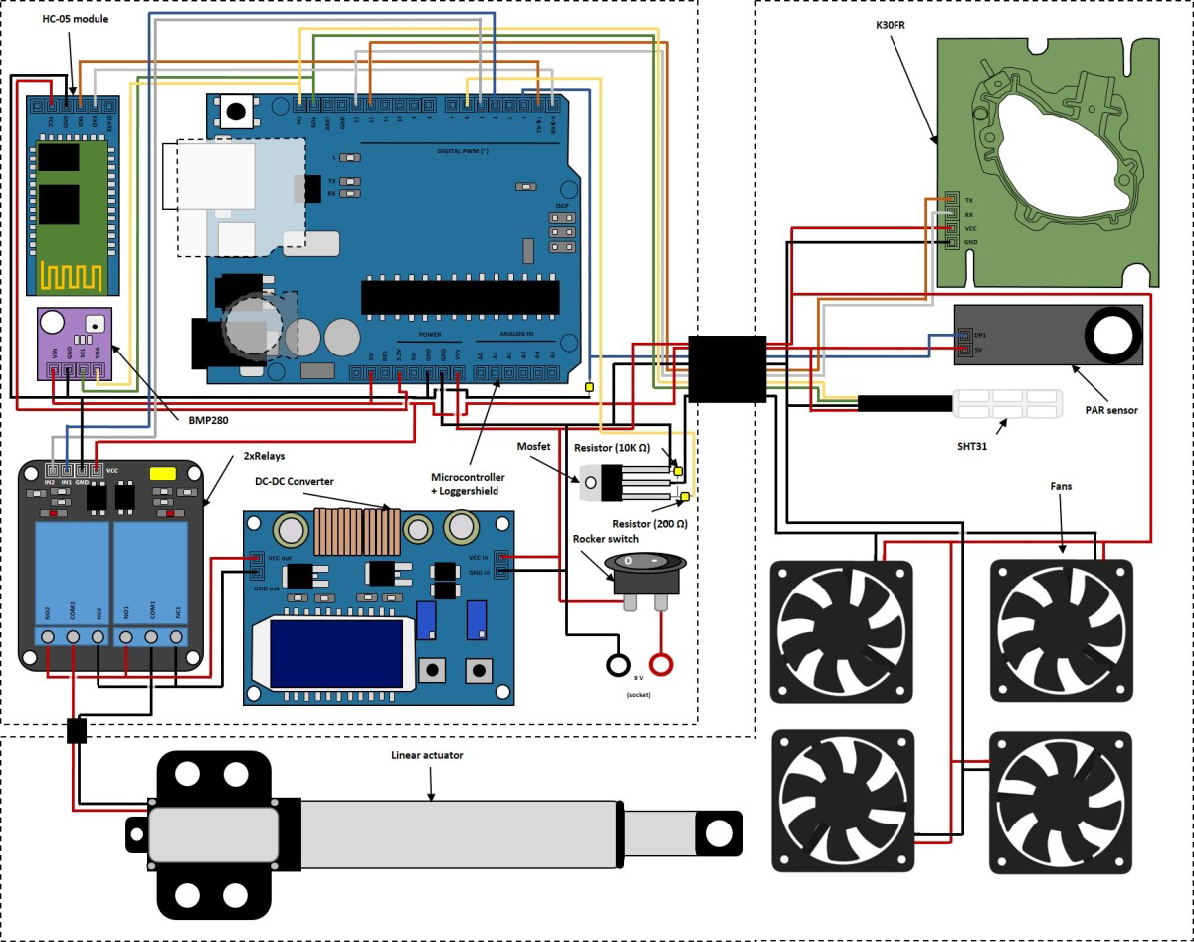
\includegraphics[keepaspectratio]{assets/mesocosm-flux-system-wiring.png}}

}

\caption{\label{fig-mesocosm_flux_system_wiring}Wiring scheme for the
mesocosm system for automatic CO2 and ET flux measurements, illustrating
the electrical connections between the microcontroller (e.g., UNO),
HC-05 Bluetooth module, data logger module, relays module, mosfet, DC-DC
converter, BMP280 module, K30FR, PAR sensor, SHT41, axial fans and
linear actuator. The schematic focuses solely on the wiring layout
required for sensor assembly, not placement of components and
additional, non-electronical components within the sensor case.}

\end{figure}%

\subsubsection{Assembly Instructions:}\label{sec-mesocosm-flux-assembly}

The following section provides a step-by-step assembly guide for
constructing the manual system to measure CO2 and ET fluxes, detailing
the integration of all components:

\begin{enumerate}
\def\labelenumi{\arabic{enumi}.}
\item
  Prepare outdoor control case (170×110×48 mm); drill two holes into the
  back wall for mounting the case to the chamber door with screws. Drill
  an additional hole at the top for the linear actuator cable and one at
  the bottom for the 9V power input.
\item
  Install connectors into the case; fit one female DC power jack socket
  at the top and one at the bottom wall. Install an 8-pin aviation
  connector on the front wall to connect sensors and fans.
\item
  Cut hard foam insert for internal compartment; use a hard foam plate
  and a carpet knife to cut one vertical and one horizontal insert,
  creating four compartments inside the case.
\item
  Fit components into the foam compartments

  \begin{enumerate}
  \def\labelenumii{\alph{enumii}.}
  \tightlist
  \item
    Microcontroller + data logger shield → upper left\\
  \item
    Step-down converter → lower left\\
  \item
    Relay module → upper right\\
  \item
    MOSFET and aviation connector wiring → lower right
  \end{enumerate}
\item
  Install ATmega328 microcontroller with data logger shield; place in
  upper-left compartment, ensuring SD card slot remains accessible.
\item
  Install 2-channel relay module; mount in upper-right compartment and
  connect:

  \begin{enumerate}
  \def\labelenumii{\alph{enumii}.}
  \tightlist
  \item
    IN1 and IN2 → microcontroller digital pins 2 and 3\\
  \item
    VCC and GND → 5V and GND from microcontroller\\
  \item
    COM1 and COM2 → top DC jack socket (actuator power)\\
  \item
    NC1 to NC2, NO1 to NO2
  \end{enumerate}
\item
  Install step-down DC converter in lower-left compartment Connect:

  \begin{enumerate}
  \def\labelenumii{\alph{enumii}.}
  \tightlist
  \item
    IN+ and IN− → 9V input from bottom DC jack\\
  \item
    OUT+ and OUT− → COM1 and COM2 on relay (to power actuator)
  \end{enumerate}
\item
  Wire the MOSFET (air exchange fan control):

  \begin{enumerate}
  \def\labelenumii{\alph{enumii}.}
  \tightlist
  \item
    Gate (G) → digital pin 7 via 10kΩ resistor\\
  \item
    Source (S) → GND (common 9V ground)\\
  \item
    Drain (D) → negative terminals of air exchange fans\\
  \item
    Add 200Ω resistor between Gate and GND
  \end{enumerate}
\item
  Mount and wire linear actuator to chamber door:

  \begin{enumerate}
  \def\labelenumii{\alph{enumii}.}
  \tightlist
  \item
    Mechanically attach actuator to sliding door\\
  \item
    Route actuator cable through top hole and connect to top DC jack
    socket
  \end{enumerate}
\item
  Install Bluetooth module (HC-05):

  \begin{enumerate}
  \def\labelenumii{\alph{enumii}.}
  \tightlist
  \item
    TX and RX → RX and TX on microcontroller (cross-wired)\\
  \item
    VCC and GND → 5V and GND on microcontroller
  \end{enumerate}
\item
  Install K30 FR and SHT31 sensors; mount sensors in a 3D-printed
  housing on the inside of the chamber door.
\item
  Install fans for air exchange and mixing:

  \begin{enumerate}
  \def\labelenumii{\alph{enumii}.}
  \tightlist
  \item
    Air exchange fans: behind sliding door (facing opposite
    directions)\\
  \item
    Mixing fans: top and bottom of chamber door
  \end{enumerate}
\item
  Wire K30 FR CO₂ sensor:

  \begin{enumerate}
  \def\labelenumii{\alph{enumii}.}
  \tightlist
  \item
    Pins 3 and 4 → digital pins 2 and 3 on microcontroller\\
  \item
    Pin 2 → 9V supply\\
  \item
    GND → GND
  \end{enumerate}
\item
  Wire fans:

  \begin{enumerate}
  \def\labelenumii{\alph{enumii}.}
  \tightlist
  \item
    Mixing fans → directly to 9V power supply\\
  \item
    Air exchange fans:

    \begin{enumerate}
    \def\labelenumiii{\roman{enumiii}.}
    \tightlist
    \item
      Positive → 9V positive\\
    \item
      Negative → MOSFET Drain
    \end{enumerate}
  \end{enumerate}
\item
  Wire SHT31 and BMP280 sensor:

  \begin{enumerate}
  \def\labelenumii{\alph{enumii}.}
  \tightlist
  \item
    SDA and SCL → I²C pins (A4/A5) on microcontroller\\
  \item
    VCC and GND → 5V and GND on microcontroller
  \end{enumerate}
\item
  Route sensor and fan cables; guide all wiring through a PG9 cable
  gland on the chamber door into the 8-pin aviation connector using
  color-coded wires for easy identification.
\item
  Secure and finalize wiring; use insulation tape or shrink tubing to
  protect all connections. Ensure neat cable management to prevent
  physical or electrical damage.
\item
  Upload program code to microcontroller and check if all system
  components deliver values in expected range via Bluetooth
\item
  Connect a 9V power supply to the bottom DC jack socket and verify that
  the linear actuator, sensors, fans, and logging of data work as
  intended.
\end{enumerate}

\subsubsection{Calibration:}\label{sec-mesocosm-flux-calibration}

Although the CO₂ and relative humidity (RH) sensors used in the
automatic chamber system provide direct output in parts per million
(ppm) and percentage (\%), regular verification of sensor performance is
recommended to ensure long-term accuracy. A practical and low-cost
method for calibrating the CO₂ sensor involves injecting a known amount
of 100\% CO₂ gas into the sealed chamber and comparing the resulting
concentration increase with the expected theoretical value based on
chamber volume and dilution principles. In the following a step by step
guide is given:

\ul{\textbf{TODO: Fix equations}}

\begin{enumerate}
\def\labelenumi{\arabic{enumi}.}
\item
  Ensure the chamber is properly sealed to avoid gas leakage during
  calibration. Check gaskets and lid tightness beforehand.
\item
  Measure the exact internal volume of the chamber (in ml).
\item
  Use a CO₂ cartridge (e.g., soda charger) with a pressure regulator and
  syringe or flow meter to inject a known volume of pure CO₂ gas into
  the chamber (e.g., 10 mL of 100\% CO₂).
\item
  Calculate the expected increase in CO₂ concentration using the
  following formula:\\
  ΔCO₂ (ppm) = (Injected CO₂ volume (ml) / Chamber volume (ml)) × 10⁶

  For example, injecting 10 mL of CO₂ into a 20 L sealed chamber would
  yield:\\
  ΔCO₂ = (10 / 20000) × 10⁶ = 500 ppm
\item
  Wait a few seconds to allow gas mixing by the fans and observe the
  sensor reading. The CO₂ sensor should register a rise in concentration
  close to the calculated value.
\item
  Stability check: After the initial rise, the CO₂ concentration should
  remain stable over several minutes. A decline suggests leakage or
  mixing issues.
\end{enumerate}

This simple test allows verification of both sensor functionality and
chamber sealing integrity and can be repeated periodically. While
relative humidity sensors are more difficult to calibrate, you can still
verify their performance by:

\begin{enumerate}
\def\labelenumi{\arabic{enumi}.}
\item
  Comparing the RH reading inside the closed chamber with a trusted
  portable hygrometer under stable ambient conditions.
\item
  Performing this check under controlled RH conditions (e.g., at early
  morning dewpoint saturation or stable indoor environment) to ensure
  consistency across devices.
\end{enumerate}

Together, these checks help validate the accuracy and operational
stability of your mesocosm system for automatic CO2 and ET flux
measurements under real-world conditions.

\subsubsection{Code:}\label{sec-mesocosm-flux-code}

Please see Arduino IDE code example given in
Section~\ref{sec-appendix_A} to implement the mesocosm system for
automatic CO2 and ET flux measurements.

\subsection{Water-stable isotope bag sampling
system}\label{sec-isotope-bag}

\subsubsection{Purpose \& Use Case:}\label{sec-isotope-bag-purpose}

Water-stable isotopes are commonly used in hydrological, ecological and
ecophysiological research. Until now, measurements were obtained either
destructive or directly in the field. Here, we present a novel,
affordable, and easy-to-use approach to measure the stable isotope
signatures of soil water (water vapor samples), thus disentangling
sampling and analyzes. Our gas bag approach demonstrates high accuracy
and extends the usability by allowing water vapor samples to be
collected and stored in the field without the need for bringing a cavity
ring-down spectroscopy (CRDS) analyzer or a permanent power supply
directly to the field. The system is based on two components: a reusable
water vapor sample bag and a dry air pump box.

\subsubsection{Bill of Materials:}\label{sec-isotope-bag-bom}

A comprehensive overview of all components required to build the
water-stable isotope bag sampling system (including one gas bag), needed
quantities, recommended suppliers and approximate prices (in €) is
provided in Table~\ref{tbl-isotope_bag_bom}.

\begin{longtable}[]{@{}
  >{\raggedright\arraybackslash}p{(\linewidth - 6\tabcolsep) * \real{0.3288}}
  >{\raggedright\arraybackslash}p{(\linewidth - 6\tabcolsep) * \real{0.2192}}
  >{\raggedright\arraybackslash}p{(\linewidth - 6\tabcolsep) * \real{0.2329}}
  >{\raggedright\arraybackslash}p{(\linewidth - 6\tabcolsep) * \real{0.2192}}@{}}
\caption{Components required for system assembly; includes quantity,
typical suppliers, and approximate prices (no links provided due to
frequent changes).}\label{tbl-isotope_bag_bom}\tabularnewline
\toprule\noalign{}
\begin{minipage}[b]{\linewidth}\raggedright
Component
\end{minipage} & \begin{minipage}[b]{\linewidth}\raggedright
Amount
\end{minipage} & \begin{minipage}[b]{\linewidth}\raggedright
Supplier
\end{minipage} & \begin{minipage}[b]{\linewidth}\raggedright
Price (approx.)
\end{minipage} \\
\midrule\noalign{}
\endfirsthead
\toprule\noalign{}
\begin{minipage}[b]{\linewidth}\raggedright
Component
\end{minipage} & \begin{minipage}[b]{\linewidth}\raggedright
Amount
\end{minipage} & \begin{minipage}[b]{\linewidth}\raggedright
Supplier
\end{minipage} & \begin{minipage}[b]{\linewidth}\raggedright
Price (approx.)
\end{minipage} \\
\midrule\noalign{}
\endhead
\bottomrule\noalign{}
\endlastfoot
Gas bag & 1 & & 20.00 € \\
Rocker switch (2 connections) & 1 & Amazon, Conrad, Reichelt & 1.00 € \\
PTFE tubing - 1/4'' outer diameter & 4 cm & Wolf-Technik eK & 0.10 € \\
PTFE tubing - 4 mm outer diameter & 6 cm & Wolf-Technik eK & 0.10 € \\
F luer-lock connection (4 mm tube) & 1 & GMPTEC GmbH & 1.00 € \\
One-way luer-lock stopcock & 1 & fisher scientific & 3.00 € \\
Two-component adhesive & - & 3M & 10.00 € \\
Hose clamp (6--12 mm) & 1 & Amazon, Conrad, Reichelt & 0.60 € \\
Transparent tape / isolation tape & 10 cm & Amazon, Conrad, Reichelt &
0.10 € \\
Parafilm & 10 cm & Carl Roth & 0.10 € \\
Tool box & 1 & Amazon, Conrad, Reichelt & 15.00 € \\
Screw top bottle with lid (1 L) & 1 & Carl Roth & 10.00 € \\
Silica gel (e.g.~orange) & 1 kg & Carl Roth & 60.00 € \\
PTFE tubing - 1/4'' outer diameter & 30 cm & Wolf-Technik eK & 0.30 € \\
PTFE tubing - 4 mm outer diameter & 300 cm & Wolf-Technik eK & 3.00 € \\
M/F luer-lock connection (1/4'' tube) & 1/1 & Carl Roth & 2.00 € \\
M/F luer-lock connection (4 mm tube) & 1/7 & GMPTEC GmbH & 1.00 € \\
One-way luer-lock stopcock & 3 & fisher scientific & 9.00 € \\
T-shaped tube connector & 2 & Amazon, Conrad, Reichelt & 4.00 € \\
Two-component adhesive & - & 3M & 10.00 € \\
Foam / Wooden planks & - & Hardware store & 10.00 € \\
Gas pump (approx. 5 L/min) & 1 & KNF & 200.00 € \\
12V Battery & 1 & Amazon, Conrad, Reichelt & 30.00 € \\
Wires (black and red) & 15 cm & Amazon, Conrad, Reichelt & 0.20 € \\
Faston connection & 2 & Amazon, Conrad, Reichelt & 0.10 € \\
One-way flow control valve (4 mm) & 3 & Reichelt & 36.00 € \\
Teflon tape & 10 cm & Amazon, Conrad, Reichelt & 0.10 € \\
Parafilm & 40 cm & Carl Roth & 0.30 € \\
Fine-mesh net & - & Amazon, Conrad, Reichelt & 1.00 € \\
Cable tie & - & Amazon, Conrad, Reichelt & 1.00 € \\
\textbf{Total} & & & \textbf{412.30 €} \\
\end{longtable}

\subsubsection{Wiring Diagram:}\label{sec-isotope-bag-wiring}

A schematic overview of the assembly and wiring layout, showing all
necessary connections between components, is provided in
Figure~\ref{fig-isotope_bag_wiring}.

\begin{figure}

\centering{

\pandocbounded{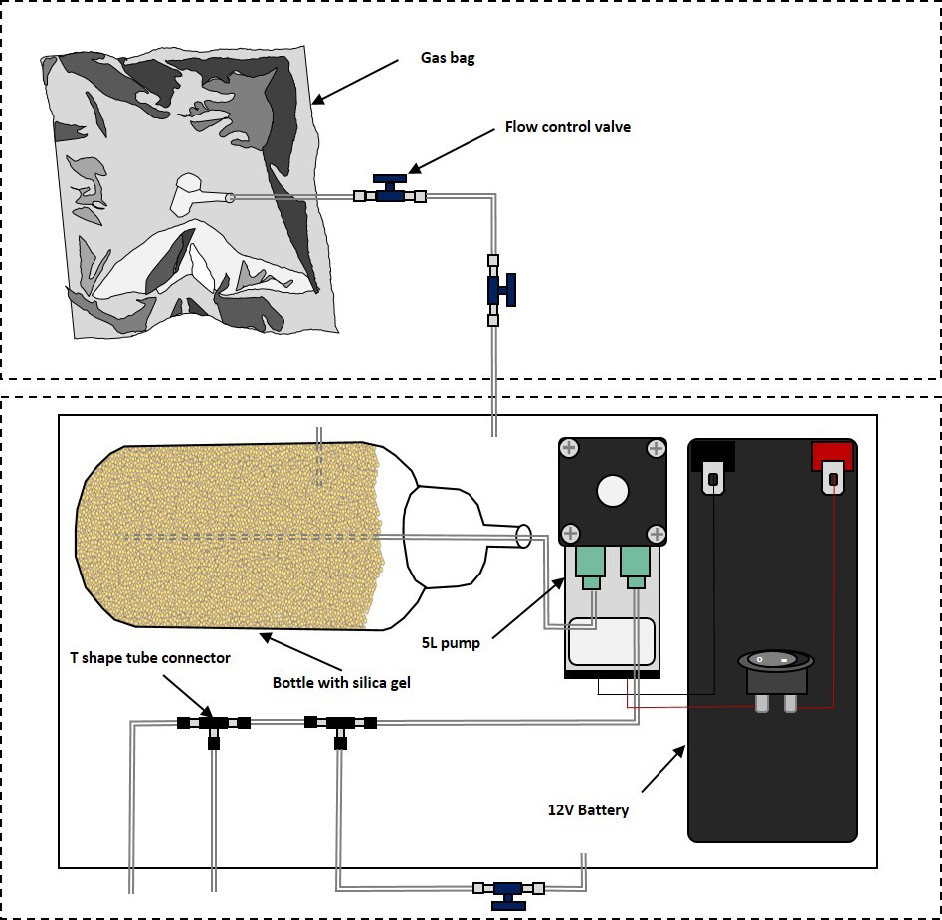
\includegraphics[keepaspectratio]{assets/isotope-bag-wiring.png}}

}

\caption{\label{fig-isotope_bag_wiring}Assembly scheme for the
water-stable isotope bag sampling system (including one gas bag),
illustrating the electrical connections between 5L pump and 12V battery
as well as tubing to the gas bag, pump and dry air supply box.}

\end{figure}%

\subsubsection{Assembly Instructions:}\label{sec-isotope-bag-assembly}

The following section provides a step-by-step assembly guide for
constructing the sample bag and additional connection, detailing the
integration of all components (the connection can be adapted for
specific use cases): unpack the gas bag

\begin{enumerate}
\def\labelenumi{\arabic{enumi}.}
\item
  slide a 4 cm long PTFE tube onto the valve of the gas bag
\item
  glue a 6 cm long 4 mm PTFE tube into the 1/4'' PTFE tube (24h drying
  time)
\item
  secure the 1/4'' PTFE tube on the valve with the hose clamp
\item
  connect a female Luer-Lock connection to the 4 mm PTFE tube
\item
  connect the 2-1 luer-lock stopcock
\item
  wrap the adhesive joint with transparent adhesive tape (only to
  prevent the adhesive joint from breaking)
\item
  wrap the adhesive joint with parafilm (only to prevent the adhesive
  joint from breaking)
\item
  secure the round tape under the valve with additional transparent tape
\end{enumerate}

The following section provides a step-by-step assembly guide for
constructing the dry air supply box, detailing the integration of all
components:

\begin{enumerate}
\def\labelenumi{\arabic{enumi}.}
\setcounter{enumi}{8}
\item
  prepare the toolbox to install all components (with wood or plastic)
\item
  attach the battery and pump in the box\\
\end{enumerate}

\begin{enumerate}
\def\labelenumi{\alph{enumi}.}
\tightlist
\item
  Connect the pump and battery with power cables (optionally with a
  switch that can be attached to the outside of the tool case)
\end{enumerate}

\begin{enumerate}
\def\labelenumi{\arabic{enumi}.}
\setcounter{enumi}{10}
\tightlist
\item
  prepare the glass bottle with desiccant (silica beads)\\
\end{enumerate}

\begin{enumerate}
\def\labelenumi{\alph{enumi}.}
\tightlist
\item
  drill a hole for the 1/4'' and 4 mm PTFE tube in the lid of the
  bottle\\
\item
  measure the 1/4'' tube distance (the tube should be placed approx. 5
  cm above the bottom of the bottle in the middle)\\
\item
  Insert a 4 mm PTFE tube into the lid hole to ensure the air supply and
  prevent the silica beads from escaping\\
\item
  Insert the 1/4'' PTFE tube into the lid and fix the fine-mesh net at
  the open end in the bottle with a cable tie to prevent the silica
  beads from entering the tube\\
\item
  Attach a tube connector to the other end
\end{enumerate}

\begin{enumerate}
\def\labelenumi{\arabic{enumi}.}
\setcounter{enumi}{11}
\item
  Connect a short piece of PTFE tubing to the pump inlet to connect the
  bottle with desiccant
\item
  connect a piece of PTFE tubing to the pump outlet\\
\end{enumerate}

\begin{enumerate}
\def\labelenumi{\alph{enumi}.}
\tightlist
\item
  Depending on the application, different numbers of outlets can be
  connected here with T-shaped hose connections (depending on the pump
  capacity)\\
\item
  Connect the control valves to regulate the flow to the outlets\\
\item
  Optional: Add a one-way luer-lock stopcock to each outlet to be able
  to close them if necessary.
\end{enumerate}

\subsubsection{Calibration and Handling
Recommendation:}\label{sec-isotope-bag-calibration}

To calibrate the measurements, a three-point standard calibration should
be used (similar to liquid water stable isotope measurements). These
standards should encompass the expected isotope range of the samples in
both directions. Our measurements over an entire cultivation period
provided many insights into the handling of the described gas bag
approach:

\begin{enumerate}
\def\labelenumi{\arabic{enumi}.}
\item
  Regarding the described dry air supply box, the use should always be
  tested for the specific application, as a very high flow rate combined
  with very humid air could greatly affect the duration of possible use.
\item
  Using the gas bags, the manufacturer states that the valves should not
  be opened more than one turn (Sense Trading B.V., personal
  communication, 2024). However, our experience has shown that a quarter
  to half opening is already sufficient to fill the gas bags reliably.
  If the gas bags are opened too wide, leaks may occur, and the sample
  may be contaminated. In addition, great care must be taken not to fill
  the bags more than 90\% to avoid material damage (as specified by the
  manufacturer). On the other hand, a larger sample is recommended to
  reduce any effect on the sample.
\item
  When using the bags in the field, it is necessary to record the source
  temperature at the corresponding depth during the measurement to be
  able to convert the isotopic signature of the soil water from vapor to
  liquid. In addition, it should be ensured that there is no liquid
  water in the soil probes, e.g.~by flushing with dry air beforehand.
  Furthermore, it is advantageous to fill the bags in a protected box to
  avoid large temperature differences in the bag during filling
  (e.g.~due to solar radiation in summer) and reduce the risk of damage
  to the gas bag, e.g.~from sharp plant parts. The same applies to
  transport.
\item
  When reusing the bags, it was important that: 1.) the bags were rinsed
  ten times with dry air, 2.) the additional connection including valve
  was built and 3.) the bags and their valves (especially the seals)
  were regularly checked for damage. To avoid holes in the bags due to
  frequent filling/emptying, areas of the bag that are heavily creased
  can be reinforced with tape to be on the safe side.
\item
  The subsequent measurement in the laboratory was easy to perform, but
  the combination of the vapor storage method with in situ probes
  requires that the temperature in the laboratory is higher than the
  source temperature during the measurement. Otherwise, condensation
  will occur in the bag, which can greatly distort the measurement
  result.
\end{enumerate}

\subsubsection{Code:}\label{sec-isotope-bag-code}

None.

\subsubsection{References}\label{sec-isotope-bag-references}

For further information see: (Dahlmann et al. 2025)

\bookmarksetup{startatroot}

\chapter{Software Solutions}\label{software-solutions}

\section{MonksHillLab Logger App}\label{sec-monkshilllab-app}

\subsection{Purpose \& Use Case:}\label{sec-monkshilllab-app-purpose}

The ``MonkshillLab Logger App'' is an Android-based tool developed to
support field deployment of low-cost DIY environmental monitoring
systems presented in this Handbook. It enables wireless Bluetooth
communication between mobile devices and DIY sensors, allowing users to
retrieve logged data or trigger new measurements directly in the field.
For systems like the handheld NDVI sensor (see
Section~\ref{sec-handheld-spectral}), the app is essential, as data are
stored solely on the mobile device. For other platforms such as the
weather station (see Section~\ref{sec-eve-platform}) and the manual
system to measure CO₂/ET fluxes (see Section~\ref{sec-manual-flux}), the
app usage is optional but provides a convenient alternative to physical
data retrieval. Beyond sensor communication, the app includes modes for
manually entering field observations---such as leaf temperature or soil
moisture. This allows users to directly digitize field data at the point
of measurement, improving organization and reducing transcription
errors. All functionalities are structured into modular ``modes'' within
the app, which users can select depending on the used low-cost DIY
system or measurement task in field.

\subsection{System
Requirements:}\label{sec-monkshilllab-app-requirements}

The ``MonkshillLab Logger App'' is developed using
\href{https://appinventor.mit.edu/}{MIT App Inventor} and is currently
available as a standalone \texttt{.apk} file (\textasciitilde3.7 MB;
Section~\ref{sec-appendix_C}). It is compatible with most Android
devices, typically Android 6.0 (Marshmallow) or higher. The app is not
available on the Google Play Store and must be downloaded manually (see
Section~\ref{sec-monkshilllab-app-installation}). For Bluetooth
communication, the app is designed to work with HC-05 Bluetooth modules,
which operate using the classic Bluetooth protocol. These modules are
commonly used in low-cost DIY microcontroller systems and are supported
by Android. iOS devices are not compatible with HC-05 modules and are
therefore not supported by the current version of the app. To ensure
proper functionality, the Android device must support:

\begin{enumerate}
\def\labelenumi{\arabic{enumi}.}
\tightlist
\item
  Classic Bluetooth (not only BLE)
\item
  External storage access, which is needed to store \texttt{.csv} files
  in download folder
\item
  Location permission, which is needed to scan for new Bluetooth devices
\end{enumerate}

\subsection{Installation \&
Setup:}\label{sec-monkshilllab-app-installation}

The ``MonkshillLab Logger App'' is distributed as a standalone
\texttt{.apk} file (see Section~\ref{sec-appendix_C}) and must be
installed manually. The file can be transferred to the Android device
via USB, Bluetooth, or email/cloud services. To install the app:

\begin{enumerate}
\def\labelenumi{\arabic{enumi}.}
\tightlist
\item
  Enable ``Install unknown apps''; On most Android devices, navigate to:
  Settings → Apps \& notifications → Special app access → Install
  unknown apps; Then allow your file manager (e.g., ``Files'' or
  ``Chrome'') to install apps.
\item
  Open the transferred \texttt{.apk} on the device and confirm the
  installation prompt
\item
  Grant necessary permissions; Upon first launch, the app will likely
  request:

  \begin{itemize}
  \tightlist
  \item
    Location access (required to scan for new Bluetooth devices)
  \item
    Storage access (to save generated \texttt{.csv} data files to your
    Downloads folder)
  \end{itemize}
\item
  Go to Bluetooth settings on your Android device and pair with the
  HC-05 device (usually named ``HC-05'' or similar; Tip: rename your
  low-cost DIY devices for better organization); default pairing PIN is
  often 1234 or 0000.
\end{enumerate}

Once installed and paired, the ``MonkshillLab Logger App'' is ready to
be used in the field. Users can select a measurement mode, connect to
the device, and begin data retrieval or manual entry.

\subsection{Usage Instructions:}\label{sec-monkshilllab-app-usage}

The ``MonkshillLab Logger App'' operates in six distinct modes, each
tailored to specific measurement tasks:

\begin{enumerate}
\def\labelenumi{\arabic{enumi}.}
\tightlist
\item
  Weather Station (EVE): Collects via Bluetooth environmental data from
  the weather station (see Section~\ref{sec-eve-platform})
\item
  CO₂ \& ET Sampling (Minion): Connects via Bluetooth to the manual
  device for CO2 and ET flux measurements (see
  Section~\ref{sec-manual-flux}) to initiate CO₂ and ET flux
  measurements and associate sampling location identifiers to the
  collected data.
\item
  NDVI Sampling (WallE): Connects via Bluetooth to the handhold NDVI
  sensor, enabling measurement initiation and adding sampling location
  identifiers to the collected data.
\item
  GC Sampling: Used during NFT-NSS closed chamber measurements for gas
  chromatography (GC) vial sampling. This mode automatically records
  sampling date and times, allows selection of vial numbers
  corresponding to specific time points (t0, t1, t2, t3, t4) sampled,
  and adds those information together with the sampling location
  identifiers to the collected data.
\item
  Analyzer Sampling: Serves as a backup protocol for multi-gas analyzer
  measurements by recording start and end times of measurements to
  facilitate matching gas analyzer data with measured sampling
  locations.
\item
  Multi-Purpose: Supports manual entry of measurements such as leaf
  temperature or soil moisture. Users can input a numeric value along
  with the sampling location identifiers; the date and time is
  automatically recorded and added.
\end{enumerate}

For modes 1 to 3, Bluetooth connectivity is required to communicate with
the respective systems.

\subsection{Output Format \&
Interpretation:}\label{sec-monkshilllab-app-output}

Each mode creates a CSV file named according to the mode and the date of
data collection, saved in the download folder of the Android device. The
CSV files include headers that identify the data columns, facilitating
interpretation and further analysis. Subsequent data collected on the
same date is appended to the existing file, ensuring continuous and
organized record-keeping.

\subsection{Troubleshooting \& Known
Issues:}\label{sec-monkshilllab-app-troubleshooting}

This section summarizes common issues encountered when using the
``MonkshillLab Logger App'' and provides practical solutions to help
ensure smooth operation and accurate data collection:

\begin{enumerate}
\def\labelenumi{\arabic{enumi}.}
\tightlist
\item
  Bluetooth Connectivity: Ensure Bluetooth is enabled on the Android
  device and the target system (EVE, Minion, WallE) is powered on and
  within range. Retry connection if connections fail. Also, make sure
  the devices have been properly paired in the Android Bluetooth
  settings before.
\item
  Zero Values for the handhold NDVI Sensor (e.g.~by completely blocking
  the lower sensor) might results in error warnings by the app as NaN
  NDVI values are calculated. Confirm proper sensor connection and
  adequate lighting conditions, and avoid measurements in situations
  likely to cause invalid readings.
\item
  \texttt{.csv} files are not saved: Verify that there is sufficient
  storage space on the Android device and that the app has permission to
  write files to your download folder. Additionally, ensure the
  \texttt{.csv} files are not open in other applications (e.g.,
  spreadsheet editors) during data collection, as this can prevent the
  app from saving new data.
\item
  Confirm the Android device's date and time settings are correct to
  ensure accurate timestamps for all recorded measurements.
\item
  Double-check all manually entered values and sampling location
  identifiers to prevent data entry errors.
\end{enumerate}

\bookmarksetup{startatroot}

\chapter{Real World Use \& Regional
Hubs}\label{real-world-use-regional-hubs}

\section{Philippine Hub -- Reuse of Pineapple
Residues}\label{philippine-hub-reuse-of-pineapple-residues}

\subsection{Location \& Context:}\label{sec-philippine-hub-location}

Philippine Hub was located on a smallholder pineapple farm near Calauan,
Laguna (14°07'49.9''N, 121°18'28.2''E), within the humid tropics of
Southeast Asia.

\begin{figure}

\centering{

\pandocbounded{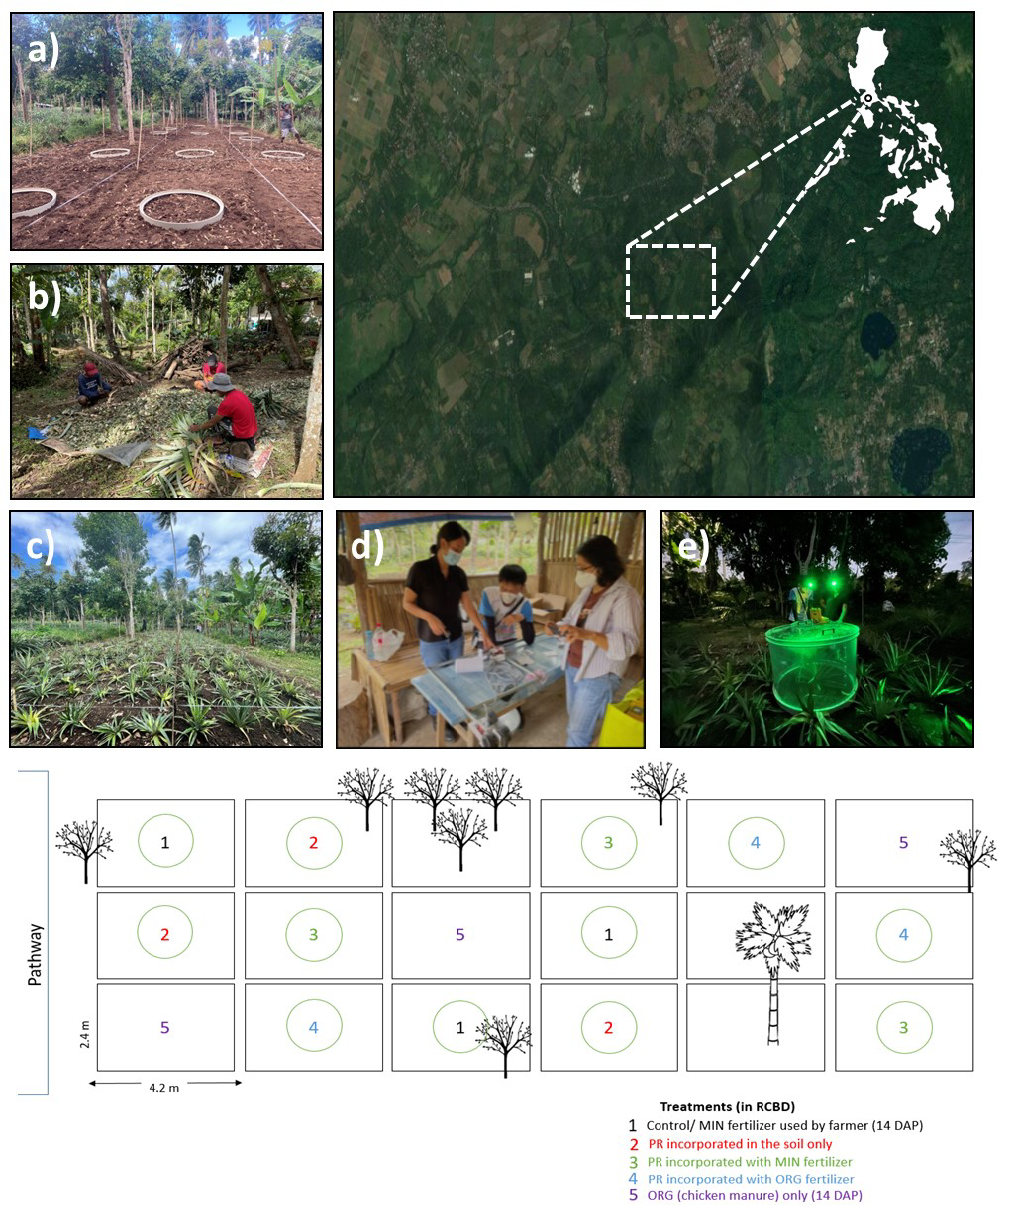
\includegraphics[keepaspectratio]{assets/philippine-hub.png}}

}

\caption{\label{fig-philippine-hub}Deployment of low-cost sensor systems
at the Philippine Hub (Calauan, Laguna, 14.13° N, 121.31° E), focusing
on the reuse of pineapple residues under different nitrogen fertilizer
strategies. (a, b, c, d, e) Field setup and sensor use on a smallholder
pineapple farm. (f) Satellite imagery showing the experimental site
location. (g) Experimental design comparing multiple residue management
and fertilizer treatments. Integrated mini weather stations and manually
operated systems were used to monitor greenhouse gas emissions (CO₂),
evapotranspiration (ET), and plant physiological responses (e.g.,
NDVI).}

\end{figure}%

From 2022 to 2023, the site hosted a field trial that tested different
reuse strategies for pineapple residues in combination with various
nitrogen (N) fertilizer forms. The research assessed their impacts on
greenhouse gas (GHG) emissions, water dynamics, carbon (C) and nitrogen
cycling, as well as crop yield. The trial addressed key challenges in
enhancing soil health and productivity in tropical smallholder systems
under resource-limited conditions.

\subsection{Used Systems:}\label{sec-philippine-hub-systems}

The handheld system for measuring spectral plant indices such as NDVI
was used alongside the manual CO₂ and ET flux measurement system
presented in this handbook. Together, these tools enabled low-cost
assessment of plant physiological responses and ecosystem gas exchange
under harsh field conditions (e.g., temperatures up to 45 °C, high
humidity, and heavy rainfall during throughout the year).

\subsection{Deployment \&
Operation:}\label{sec-philippine-hub-deployment}

The field trial was a key activity of the BMEL-funded project rePRISING,
coordinated by Reena Macagga (PhD student at ZALF and
Humboldt-Universität zu Berlin) in collaboration with the University of
the Philippines Los Baños and a local farmer. Conducted from 2022 to
2023, the field trial covered a full pineapple crop growth period,
lasting nearly 18 months on a smallholder farm near Calauan, Laguna. All
measurements---using handheld systems for spectral plant indices and
manual gas flux chambers for CO₂ and ET---were carried out on a biweekly
basis during intensive field campaigns. Mini climate stations were
installed permanently to ensure continuous environmental monitoring
throughout the field trial.

\subsection{Current Status:}\label{sec-philippine-hub-status}

The field trial has been completed. A key outcome was that the addition
of chopped pineapple residues into the soil prior to planting
substantially increased yields across all treatments---unfertilized,
mineral fertilized, and organically fertilized (chicken manure). During
a farmer workshop, participants also noted that pineapples grown with
residue addition tasted sweeter, though this observation remains
subjective and unverified by compositional analysis. Improved plant
performance was reflected in higher CO₂ exchange and NDVI values. No
consistent differences in evapotranspiration (ET) or water use
efficiency (WUE) were observed. A central achievement of this trial was
the development and successful testing of both used sensor systems under
real field conditions.

\subsection{References}\label{sec-philippine-hub-references}

For further information see: Macagga et al. (2024); Macagga et al.
(2025)

\section{Northern Ghana Hub -- Moist Savannah Dryland Rotation
Trial}\label{northern-ghana-hub-moist-savannah-dryland-rotation-trial}

\subsection{Location \& Context:}\label{sec-ghana-hub-location}

The Northern Ghana Hub is located in the moist savannah zone of Ghana
(9.41°N, -0.99°E) and was established in May 2025 at the CSIR-Savanna
Agricultural Research Institute experimental field.

\begin{figure}

\centering{

\pandocbounded{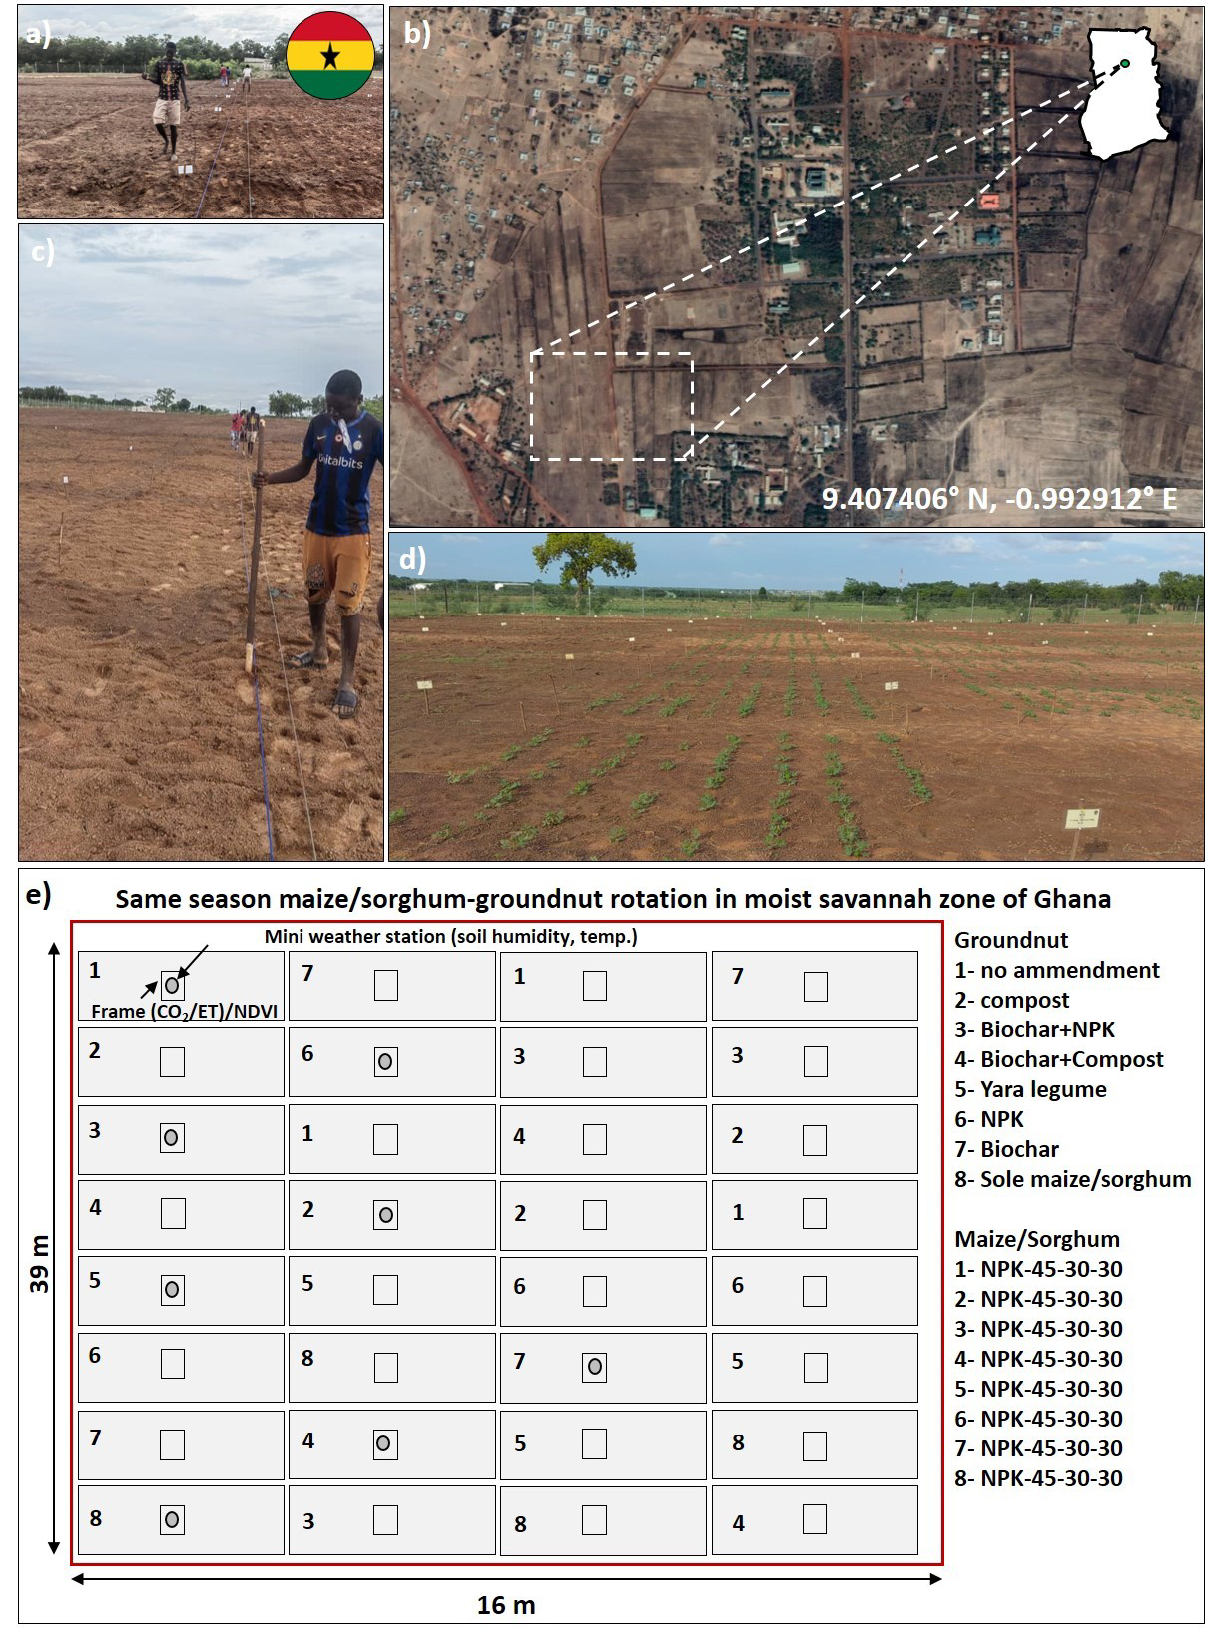
\includegraphics[keepaspectratio]{assets/ghana-hub.png}}

}

\caption{\label{fig-ghana-hub}Deployment of low-cost sensor systems at
the Northern Ghana Hub (Nyankpala, 9.41° N, -0.99° E), focusing on
sustainable same season groundnut- sorghum and groundnut- maize
rotations under different soil amendment strategies in the moist
savannah zone. (a, c, d) Field establishment and sensor installation.
(b) Satellite imagery showing experimental site location. (e)
Experimental design with eight treatment combinations including compost,
biochar, NPK fertilizers. Integrated mini weather stations and installed
frames are used to monitor gas exchange (CO2, ET and N2O) as well as
plant development and health status (e.g., NDVI).}

\end{figure}%

It aims to investigate the effect of same season groundnut-maize/sorghum
crop rotation under different soil amendments and fertilizer strategies
on GHG emissions, water, N and C cycling. It thus especially reflecting
the pressures of nutritious food production in semi-arid environments.

\subsection{Used Systems:}\label{sec-ghana-hub-systems}

The handheld system for measuring spectral plant indices such as NDVI
and PRI is used alongside the manual CO₂ and ET flux measurement system
presented in this handbook. Together, these tools enable low-cost
assessment of plant physiological responses and ecosystem gas exchange
under harsh field conditions (e.g., temperatures up to 50 °C, high
humidity, and heavy rainfall during the rainy season).

\subsection{Deployment \& Operation:}\label{sec-ghana-hub-deployment}

The field trial is operated by Dr.~Michael Asante from the CSIR--Savanna
Agricultural Research Institute in Tamale, Ghana, with support from the
Leibniz Centre for Agricultural Landscape Research (ZALF). It is planned
to run the field trial for three consecutive cropping seasons.
Measurements are scheduled on a weekly basis for spectral plant indices
(e.g., NDVI) and biweekly (twice per month) for CO₂, N2O and ET fluxes.
Deployment in the field takes place during measurement campaigns only,
except for the mini climate stations, which remain installed
continuously.

\subsection{Current Status:}\label{sec-ghana-hub-status}

Both used systems have been successfully introduced and tested under
field conditions. Weekly and biweekly measurement routines are being
established, and initial data collection has begun. While still in the
early phase, the setup has proven feasible under the local climate
Macagga et al. (2024). Continuous coordination between CSIR-SARI and
ZALF ensures technical support and protocol alignment. Full data
evaluation will follow after the first cropping season.

\subsection{References}\label{sec-ghana-hub-references}

No published references are available yet, as the research is ongoing.
Relevant outputs will be added in future handbook updates.

\section{Central Benin Hub -- Alternate Wetting and Drying Rice
Trial}\label{central-benin-hub-alternate-wetting-and-drying-rice-trial}

\subsection{Location \& Context:}\label{sec-benin-hub-location}

The Central Benin Hub is located in the moist savannah zone of Benin
(7.24°N, 2.28°E) and was established in November 2021 at the National
Water Institute experimental field.

\begin{figure}

\centering{

\pandocbounded{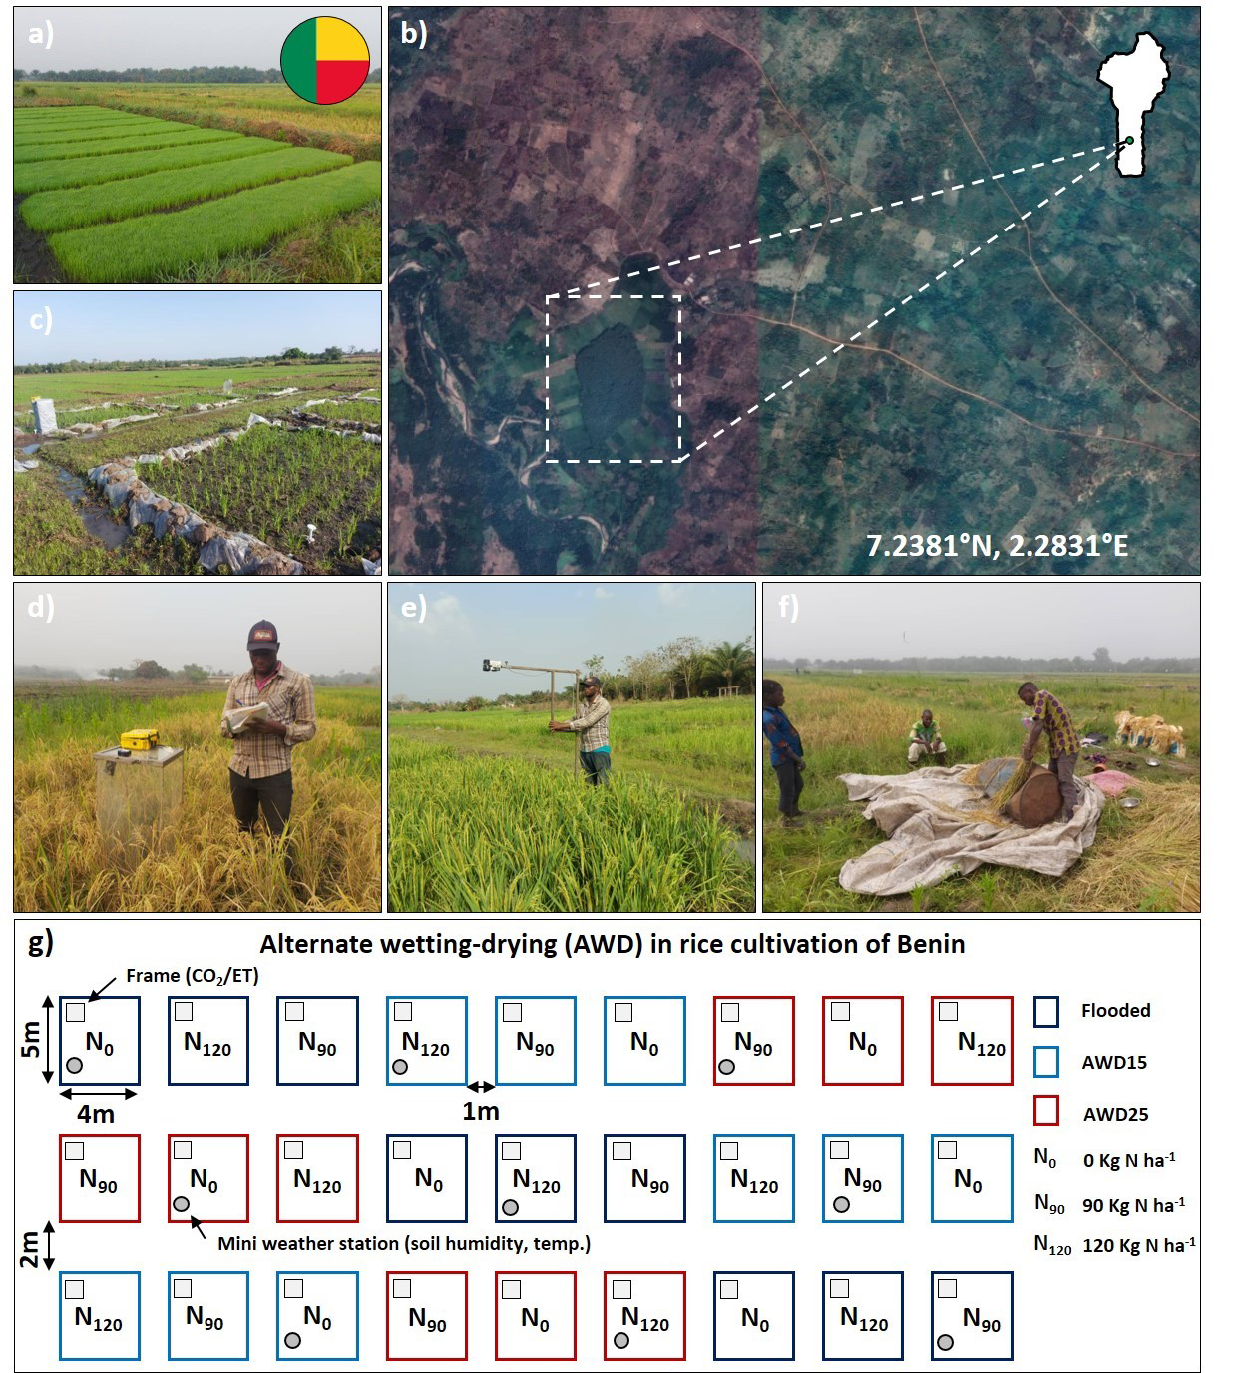
\includegraphics[keepaspectratio]{assets/benin-hub.png}}

}

\caption{\label{fig-benin-hub}Deployment of low-cost sensor systems at
the Central Benin Hub (near Koussin-Lélé; 7.24° N, 2.28° E), focusing on
sustainable wet rice cultivation under alternate wetting and drying
(AWD) practices and varying N fertilization levels in a semi-arid
environment. (a, c, d, e, f) Field establishment and sensor
installation. (b) Satellite imagery showing experimental site location.
(g) Experimental design includes six treatment combinations differing in
AWD intensity and nitrogen input. Integrated mini weather stations,
low-cost gas exchange systems (CO₂ and ET), and sensor frames are used
to monitor GHG emissions and plant physiological responses (e.g., NDVI),
supporting the development of water- and nutrient-efficient rice
production strategies.}

\end{figure}%

It aims to investigate the effect of alternate wetting and drying as
well as different N fertilization rates on GHG emissions, water, N and C
cycling of wet rice cultivation. Located in Central Benin, this hub
reflects the need for sustainable intensification and the purposeful use
of scarce water resources in the context of nutritious food production
under semi-arid conditions. It thus especially reflecting the pressures
of nutritious food production in semi-arid environments.

\subsection{Used Systems:}\label{sec-benin-hub-systems}

The handheld system for measuring spectral plant indices such as NDVI
and PRI was used alongside the manual CO₂ and ET flux measurement system
presented in this handbook. Together, these tools enable low-cost
assessment of plant physiological responses and ecosystem gas exchange
under harsh field conditions (e.g., temperatures up to 50 °C, high
humidity, and heavy rainfall during the rainy season).

\subsection{Deployment \& Operation:}\label{sec-benin-hub-deployment}

The field trial is operated by Dr.~Goeffroy Sossa from the National
Water Institute, University of Abomey-Calavi, Abomey-Calavi, Benin, with
support from the Leibniz Centre for Agricultural Landscape Research
(ZALF). The field trial was running for two consecutive cropping seasons
from 2021 to 2023. Measurements were scheduled on a weekly basis for
spectral plant indices (e.g., NDVI) and biweekly (twice per month) for
CO₂ and ET fluxes. Deployment in the field took place during measurement
campaigns only, except for the mini climate stations, which remained
installed continuously. The new set up of the field trial is planned for
November 2025 (this time running over three seasons), with the aim to
use low-cost DIY equipment, for precision timing of fertilization and
irrigation events.

\subsection{Current Status:}\label{sec-benin-hub-status}

The field trial has been completed, and the collected data have been
evaluated and submitted for publication (Sossa et al. 2024). The
analysis revealed clear difference in yield and, in particular, water
use efficiency (WUE) across the three alternate wetting and drying (AWD)
practices and two N fertilization levels. Notably, moderate AWD down to
a soil water table depth of 15 cm achieved yields comparable to
permanent flooding while significantly improving WUE. Furthermore,
increasing N input beyond a certain threshold did not lead to
substantial yield gains, highlighting the importance of timing and
resource-efficient management.

\subsection{References}\label{sec-benin-hub-references}

For more information see: Sossa et al. (2024)

\bookmarksetup{startatroot}

\chapter*{References}\label{references}
\addcontentsline{toc}{chapter}{References}

\markboth{References}{References}

\protect\phantomsection\label{refs}
\begin{CSLReferences}{1}{1}
\bibitem[\citeproctext]{ref-dahlmann2025}
Dahlmann, Adrian, John D. Marshall, David Dubbert, Mathias Hoffmann, and
Maren Dubbert. 2025. {``Simple Water Vapor Sampling for Stable Isotope
Analysis Using Affordable Valves and Bags.''} \emph{Atmospheric
Measurement Techniques} 18 (12): 2607--18.
\url{https://doi.org/10.5194/amt-18-2607-2025}.

\bibitem[\citeproctext]{ref-macagga2024}
Macagga, Reena, Michael Asante, Geoffroy Sossa, Danica Antonijević,
Maren Dubbert, and Mathias Hoffmann. 2024. {``Validation and Field
Application of a Low-Cost Device to Measure CO {\textsubscript{2}} and
Evapotranspiration (ET) Fluxes.''} \emph{Atmospheric Measurement
Techniques} 17 (4): 1317--32.
\url{https://doi.org/10.5194/amt-17-1317-2024}.

\bibitem[\citeproctext]{ref-macagga2025}
Macagga, Reena, Geoffroy Sossa, Yvonne Ayaribil, et al. 2025. {``A New,
Low-Cost Ground-Based NDVI Sensor for Manual and Automated Crop
Monitoring.''} \emph{Smart Agricultural Technology} 11 (August): 100892.
\url{https://doi.org/10.1016/j.atech.2025.100892}.

\bibitem[\citeproctext]{ref-sossa2024}
Sossa, Geoffroy, Mathias Hoffmann, Jesse Naab, et al. 2024.
\emph{Optimize Irrigated Rice Cultivation in West Africa~by Improving
Water Use Efficiency}. \url{http://dx.doi.org/10.2139/ssrn.4860972}.

\end{CSLReferences}

\bookmarksetup{startatroot}

\chapter*{Abbreviations}\label{abbreviations}
\addcontentsline{toc}{chapter}{Abbreviations}

\markboth{Abbreviations}{Abbreviations}

\textbf{PTFE}: Polytetrafluoroethylene

\textbf{PAR}: Photosynthetic Active Radiation

\textbf{BWP34}: Photodiode

\textbf{GND}: Grounding line

\textbf{5V}: 5V power line

\textbf{A2}: Analog signal line

\textbf{ET}: Evapotranspiration

\textbf{CO2}: Carbon dioxide

\textbf{CH4}: Methane

\textbf{NDVI:} Normalized Difference Vegetation index

\textbf{PRI:} Photochemical Reflectance Index

\textbf{NiMH:} Nickel-Metal Hydride

\textbf{mAh:} Milliampere hour

\bookmarksetup{startatroot}

\chapter{Appendices}\label{appendices}

\section{Appendix A --- Full Code Listings}\label{sec-appendix_A}

Complete Arduino IDE scripts, click the links download the .ino files,
or copy and paste the code blocks into your Arduino IDE.

The following Arduino IDE scripts are included in the Zenodo uploads and
are also downloadable via the links below from the Github repository for
this project. They are also available in the GitHub repository for this
project under the folder
\texttt{X\_Appendix\_A\_full\_code\_listings/}.:

\begin{enumerate}
\def\labelenumi{\arabic{enumi}.}
\item
  \href{https://github.com/zalf-lli/LCSfFE-handbook/blob/main/X_Appendix_A_full_code_listings/Automatic_NDVI/Automatic_NDVI.ino}{Automatic\_NDVI.ino}
\item
  \href{https://github.com/zalf-lli/LCSfFE-handbook/blob/main/X_Appendix_A_full_code_listings/Manual_System_CO2_ET_fluxes/Manual_System_CO2_ET_fluxes\%20.ino}{Manual\_System\_CO2\_ET\_fluxes.ino}
\item
  \href{https://github.com/zalf-lli/LCSfFE-handbook/blob/main/X_Appendix_A_full_code_listings/EVE_offline/EVE_offline_weather_station.ino}{EVE\_offline\_weather\_station.ino}
\item
  \href{https://github.com/zalf-lli/LCSfFE-handbook/blob/main/X_Appendix_A_full_code_listings/EVE_online/EVE_online_weather_station.txt}{EVE\_online\_weather\_station.txt}
\item
  \href{https://github.com/zalf-lli/LCSfFE-handbook/blob/main/X_Appendix_A_full_code_listings/Mesocosm_System.ino}{Mesocosm\_System.ino}
\end{enumerate}

\section{Appendix B --- 3D-printing/PCB board
files}\label{sec-appendix_B}

3D-printing STL files and PCB design archives for building the sensor
systems.

The following 3D-printing STL files and PCB design archives are included
in the Zenodo uploads and are also downloadable via the links below from
the Github repository for this project. They are also available in the
GitHub repository for this project under the folder
\texttt{X\_Appendix\_B\_3D\_printing\_PCB\_board\_files/}.:

\begin{enumerate}
\def\labelenumi{\arabic{enumi}.}
\item
  \href{https://github.com/zalf-lli/LCSfFE-handbook/blob/main/X_Appendix_B_3D_printing_PCB_board_files/PAR_Sensor_case.stl}{PAR\_Sensor\_case.stl}
\item
  \href{https://github.com/zalf-lli/LCSfFE-handbook/blob/main/X_Appendix_B_3D_printing_PCB_board_files/NDVI_PRI_Sensor_case.stl}{NDVI\_PRI\_Sensor\_case.stl}
\item
  \href{https://github.com/zalf-lli/LCSfFE-handbook/blob/main/X_Appendix_B_3D_printing_PCB_board_files/Automatic_NDVI_System_case_I.stl}{Automatic\_NDVI\_System\_case\_I.stl}
\item
  \href{https://github.com/zalf-lli/LCSfFE-handbook/blob/main/X_Appendix_B_3D_printing_PCB_board_files/Automatic_NDVI_System_case_II.stl}{Automatic\_NDVI\_System\_case\_II.stl}
\item
  \href{https://github.com/zalf-lli/LCSfFE-handbook/blob/main/X_Appendix_B_3D_printing_PCB_board_files/Automatic_NDVI_AS7262_3_case.stl}{Automatic\_NDVI\_AS7262\_3\_case.stl}
\item
  \href{https://github.com/zalf-lli/LCSfFE-handbook/blob/main/X_Appendix_B_3D_printing_PCB_board_files/Manual_CO2_ET_System_K30_FR_sensor_case.stl}{Manual\_CO2\_ET\_System\_K30\_FR\_sensor\_case.stl}
\item
  \href{https://github.com/zalf-lli/LCSfFE-handbook/blob/main/X_Appendix_B_3D_printing_PCB_board_files/EVE_PAR_sensor_case.stl}{EVE\_PAR\_sensor\_case.stl}
\item
  \href{https://github.com/zalf-lli/LCSfFE-handbook/blob/main/X_Appendix_B_3D_printing_PCB_board_files/EVE_SHT41_case.stl}{EVE\_SHT41\_case.stl}
\item
  \href{https://github.com/zalf-lli/LCSfFE-handbook/blob/main/X_Appendix_B_3D_printing_PCB_board_files/Automatic_NDVI_PRI_System_PCB.zip}{Automatic\_NDVI\_PRI\_System\_PCB.zip}
\item
  \href{https://github.com/zalf-lli/LCSfFE-handbook/blob/main/X_Appendix_B_3D_printing_PCB_board_files/Manual_CO2_ET_System_PCB.zip}{Manual\_CO2\_ET\_System\_PCB.zip}
\item
  \href{https://github.com/zalf-lli/LCSfFE-handbook/blob/main/X_Appendix_B_3D_printing_PCB_board_files/NiMH_Solar_Trickle_Charger_PCB.zip}{NiMH\_Solar\_Trickle\_Charger\_PCB.zip}
\item
  \href{https://github.com/zalf-lli/LCSfFE-handbook/blob/main/X_Appendix_B_3D_printing_PCB_board_files/EVE_Weather_station.zip}{EVE\_Weather\_station.zip}
\end{enumerate}

\section{Appendix C --- Other Software}\label{sec-appendix_C}

Additional software components including mobile applications, database
schemas, and backend dashboard scripts. Click the links below to
download the files from the GitHub repository for this project, or
access them in the GitHub repository under the folder
\texttt{X\_Appendix\_C\_other\_software/}.

The following software components are available in the Zenodo uploads
and are also downloadable via the links below from the Github repository
for this project. They are also available in the GitHub repository for
this project under the folder
\texttt{X\_Appendix\_C\_other\_software/}.:

\begin{enumerate}
\def\labelenumi{\arabic{enumi}.}
\item
  \href{https://github.com/zalf-lli/LCSfFE-handbook/blob/main/X_Appendix_C_other_software/MonksHillLab_Logger_APP.apk}{MonksHillLab\_Logger\_APP.apk}
\item
  \href{https://github.com/zalf-lli/LCSfFE-handbook/tree/main/X_Appendix_C_other_software/Dashboard_Backend_Scripts}{Dashboard\_Backend\_Scripts}
\item
  \href{https://github.com/zalf-lli/LCSfFE-handbook/blob/main/X_Appendix_C_other_software/SQL_scheme.txt}{SQL\_scheme.txt}
\end{enumerate}

\section{Appendix D --- Supporting Data}\label{sec-appendix_D}

Supporting datasets from field deployments and sensor comparison tests.
Click the links below to download the files from the GitHub repository
for this project, or access them in the GitHub repository under the
folder \texttt{X\_Appendix\_D\_Supporting\_Data/}.

The following datasets are available in the Zenodo uploads and are also
downloadable via the links below from the Github repository for this
project. They are also available in the GitHub repository for this
project under the folder \texttt{X\_Appendix\_D\_Supporting\_Data/}.:

\begin{enumerate}
\def\labelenumi{\arabic{enumi}.}
\item
  \href{https://github.com/zalf-lli/LCSfFE-handbook/blob/main/X_Appendix_D_Supporting_Data/36h_PAR_comparison_test.csv}{36h\_PAR\_comparison\_test.csv}
  --- 36-hour PAR sensor comparison test data
\item
  \href{https://github.com/zalf-lli/LCSfFE-handbook/blob/main/X_Appendix_D_Supporting_Data/48h_PAR_comparison_test.csv}{48h\_PAR\_comparison\_test.csv}
  --- 48-hour PAR sensor comparison test data
\item
  \href{https://github.com/zalf-lli/LCSfFE-handbook/blob/main/X_Appendix_D_Supporting_Data/EVE_Offline_Field_Deployment.csv}{EVE\_Offline\_Field\_Deployment.csv}
  --- EVE offline weather station field deployment data
\item
  \href{https://github.com/zalf-lli/LCSfFE-handbook/blob/main/X_Appendix_D_Supporting_Data/EVE_Online_Field_Deployment.csv}{EVE\_Online\_Field\_Deployment.csv}
  --- EVE online weather station field deployment data
\end{enumerate}


\backmatter


\end{document}
